\chapter{The CMS detector}
\label{sec:02_cms}

\section{Overview}

The experimental apparatus used in this dissertation is the Compact Muon Solenoid (CMS) detector (Figure~\ref{fig:02_cms_detector}), one of the two general-purpose detectors at the LHC.
It is uniquely characterized by its strong, superconducting 3.8\unit{T} solenoid magnet, around which are arranged several subdetectors to measure the properties of particles produced in collisions at the LHC.
% It comprises a superconducting 3.8\unit{T} solenoid magnet and several subdetectors to measure the properties of particles produced in proton-proton as well as, to a lesser extent, heavy-ion collisions at the LHC.
Inside the solenoid, it contains an all-silicon tracker, to measure the momenta of charged particles and identify the collision vertex, and lead-tungstate crystal electromagnetic and brass and scintillator hadronic calorimeters to measure the energy of particles interacting through the electromagnetic and strong forces, respectively.
Finally, outside the solenoid are gas-ionization detectors, interleaved with steel flux-return yoke plates, to track muons.

\begin{figure}[ht]
    \centering
    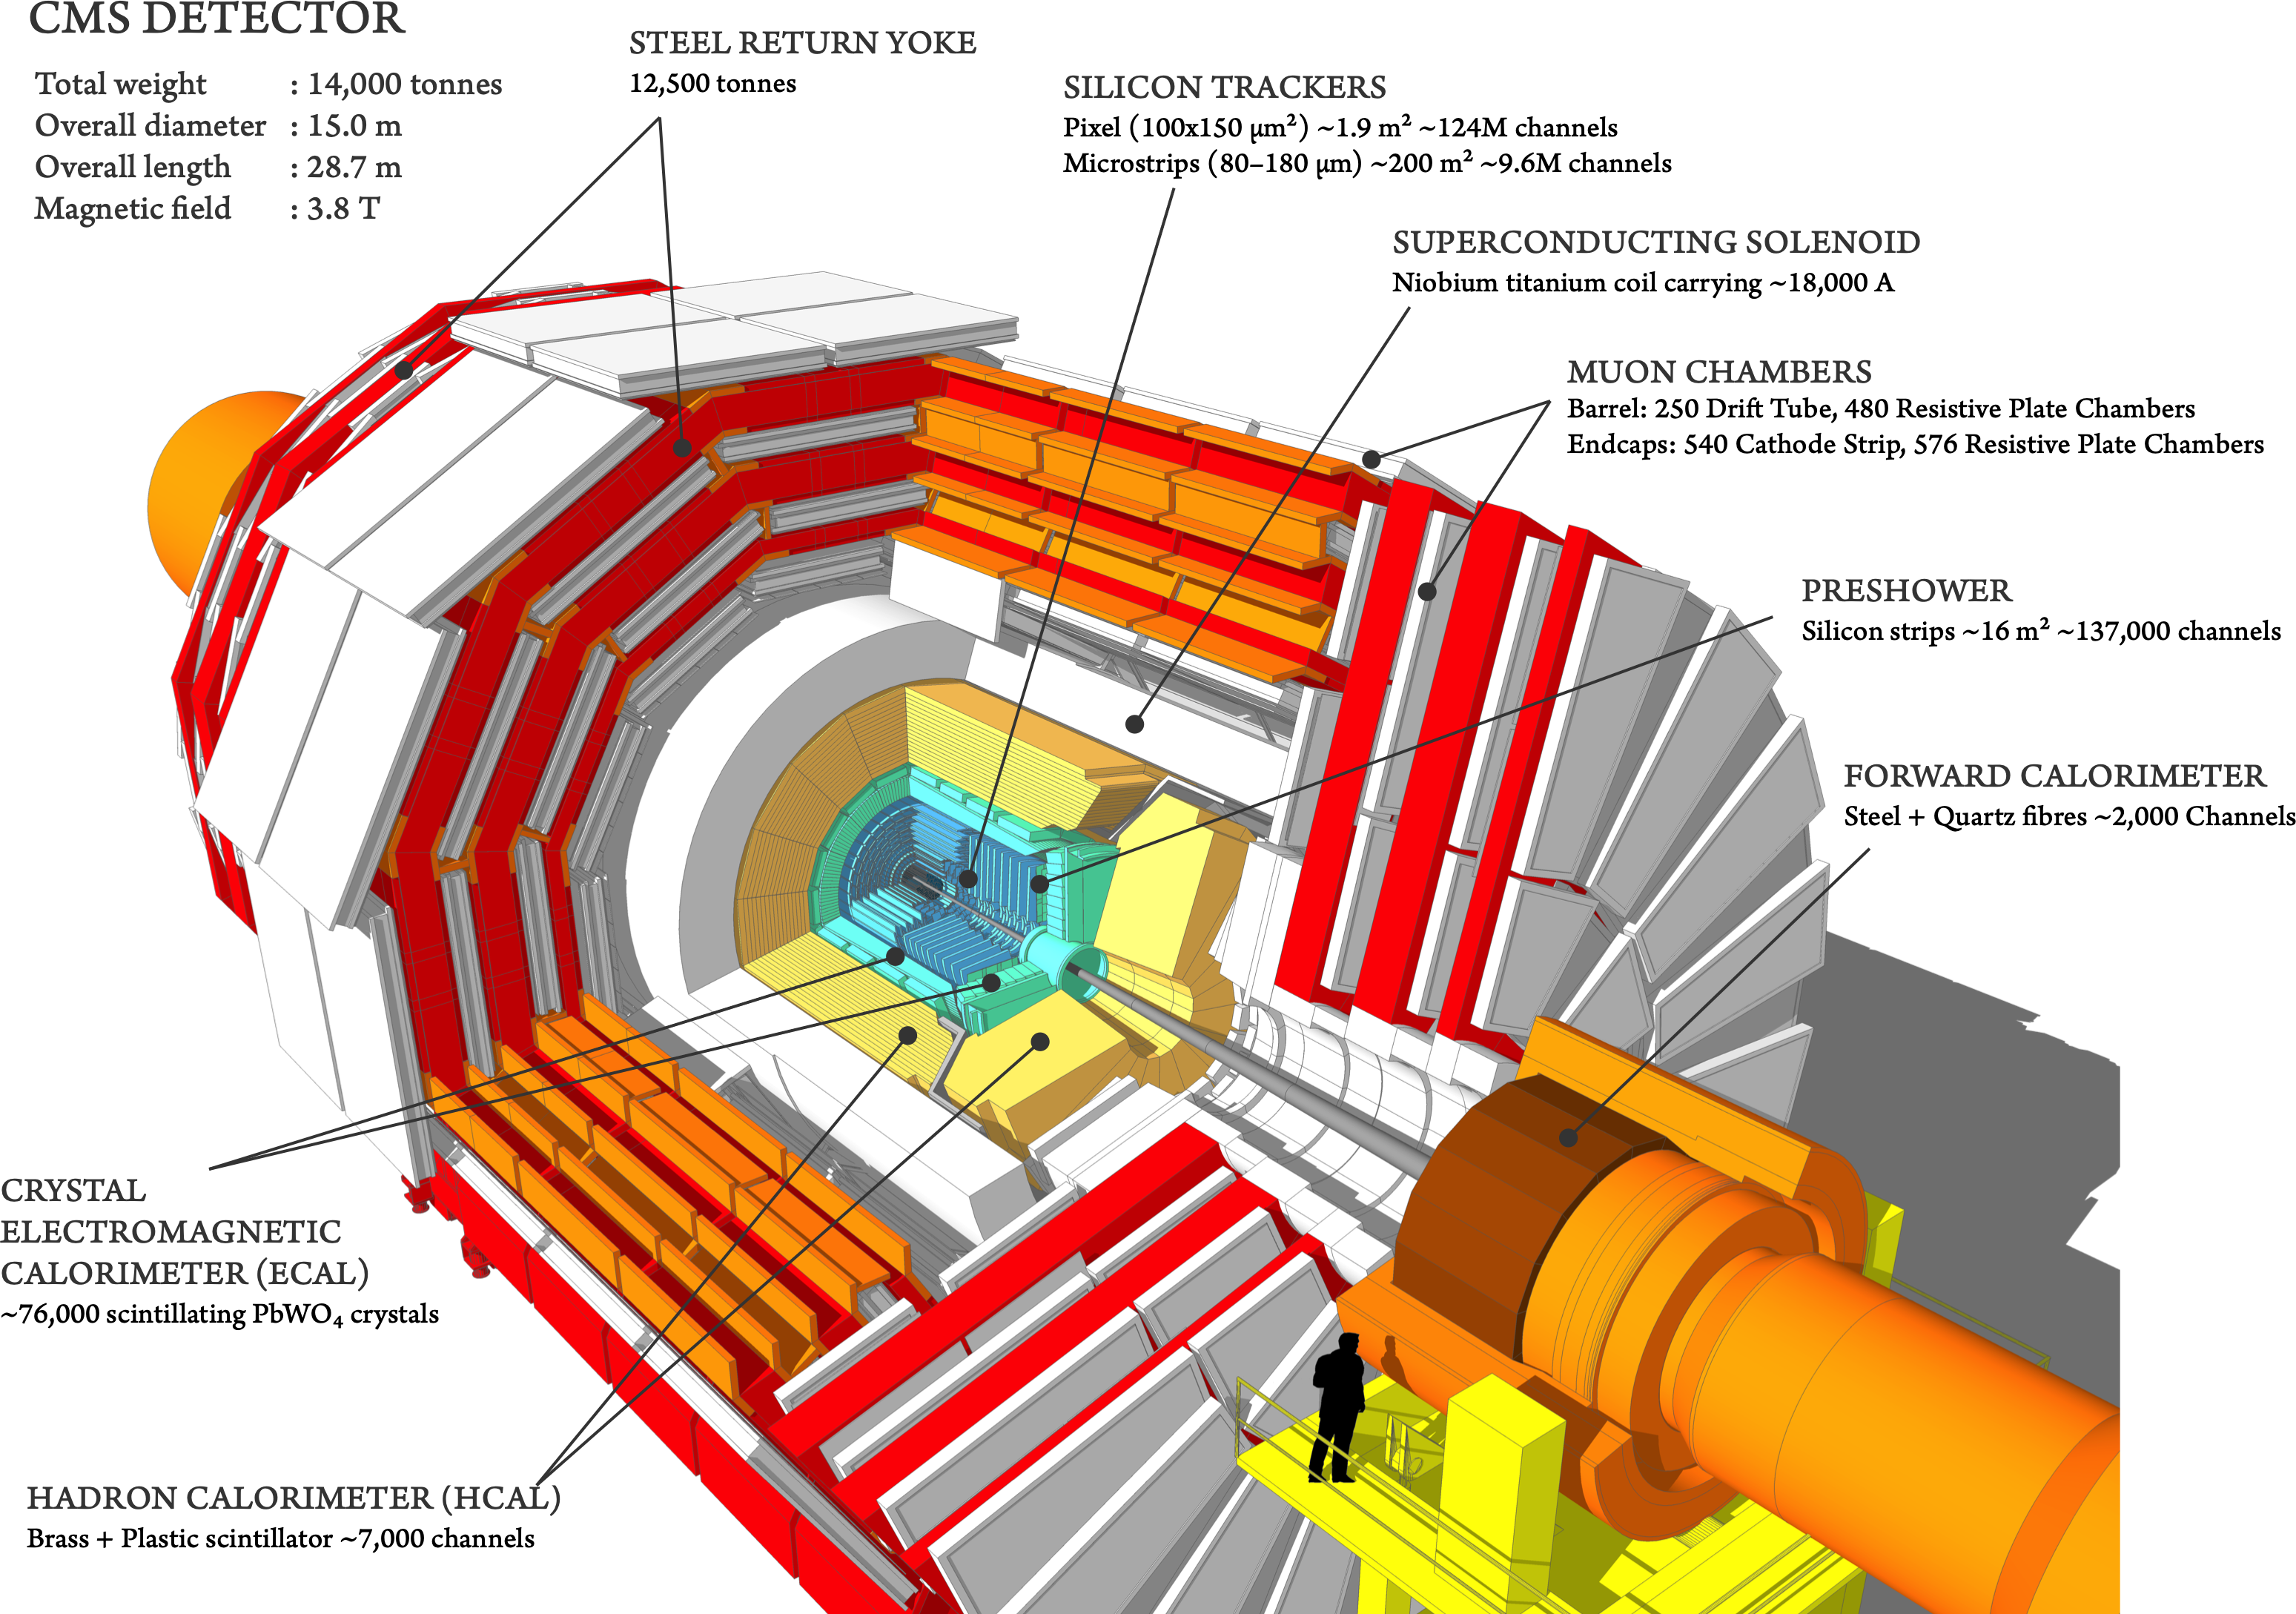
\includegraphics[width=\textwidth]{figures/02-CMS/cms/cms_schematic.png}
    \caption{A cutaway view of the CMS detector showing the various subdetectors and the solenoid magnet, reproduced from Ref.~\cite{CMS:2023gfb}.}
    \label{fig:02_cms_detector}
\end{figure}

% \begin{figure}[ht]
%     \centering
%     \captionsetup{justification=centering}
%     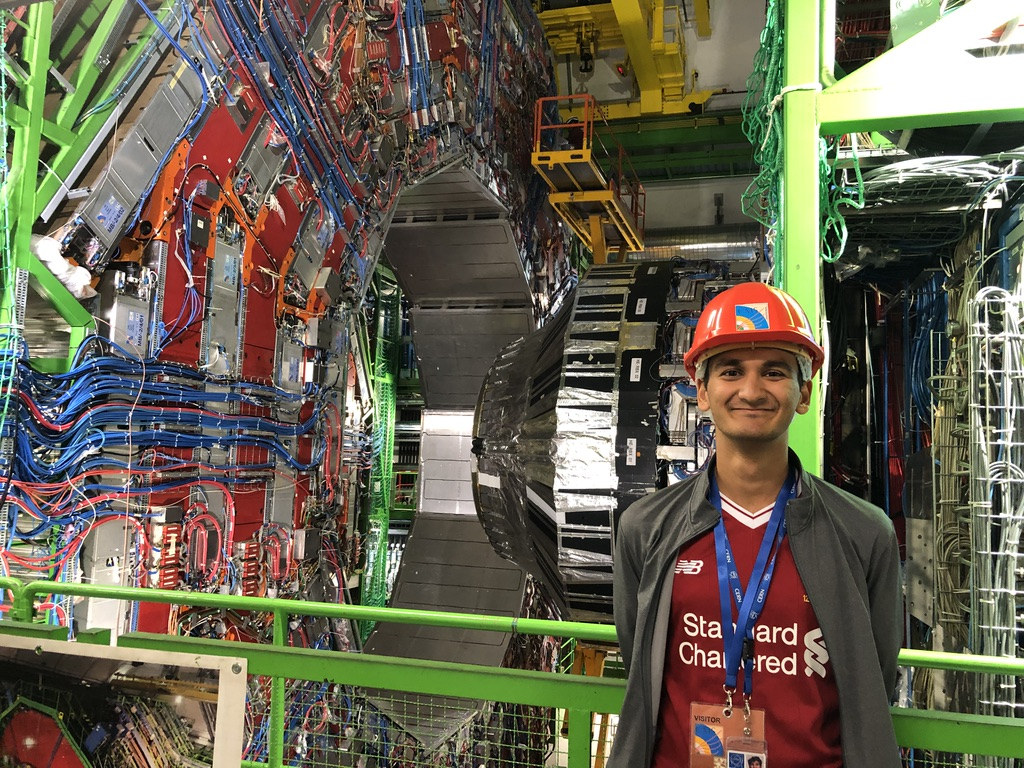
\includegraphics[width=\textwidth]{figures/02-CMS/cms/cms_raghav}
%     \caption{Author of the dissertation in front of the CMS detector in 2019.}
%     \label{fig:02_cms_raghav}
% \end{figure}

The CMS detector design was strongly motivated by the potential for discovery of the Higgs boson as well as new physics at the \TeV energy scale.
Specifically, the original design requirements were~\cite{CMS:2008xjf}:
\begin{itemize}
    \item Strong muon identification and momentum resolution, as well as good charge determination below $p < 1\TeV$;
    \item High charged-particle momentum resolution and reconstruction efficiency;
    \item Efficient triggering and good offline reconstruction of $\tau$-leptons and $b$-jets;
    \item Strong and hermetic electromagnetic energy resolution for photons and electrons;
    \item Good missing transverse energy (MET) and jet mass resolutions.
\end{itemize}
In addition to the above, the detector also had to be robust against the high radiation environment and pileup at the LHC, as well as have a powerful online event selection system, called the \textit{trigger}, to reduce the high raw 40\unit{MHz} data rate to something manageable for offline storage and analysis.

To satisfy the latter, events of interest in CMS are selected using a two-tiered trigger system.
The first level (L1) uses custom hardware processors and information from the calorimeters and muon detectors to select events at a rate of around 100\unit{kHz} within a fixed latency of 4\unit{\mus}~\cite{CMS:2020cmk}.
The second level, known as the high-level trigger (HLT), consists of a farm of processors running a version of the full event reconstruction software optimized for fast processing and reduces the event rate to around 1\unit{kHz} before data storage~\cite{CMS:2016ngn}.
Both online and offline, the raw detector signals are processed and reconstructed first locally as hits in the individual subdetectors, then as tracks and calorimeter clusters, and finally as physics objects such as electrons, muons, jets, and missing energy using the particle-flow (PF) algorithm~\cite{CMS:2017yfk}.

As we describe below, the CMS detector was able and continues to meet these ambitious requirements.
The CMS collaboration not only discovered the Higgs boson in 2012~\cite{CMS:2012qbp}, but also has since performed a wide range of measurements of the Higgs sector and the SM as well as searches for diverse new physics, such as those described in this dissertation.

Looking ahead, however, the upcoming high-luminosity era of the LHC (Chapter~\ref{sec:02_lhc_luminosity}) will bring forth considerable new challenges to the detector, with significantly higher radiation levels, occupancies, and pileup.
To overcome them, nearly all CMS subdetectors will undergo a major upgrade after Run 3, known as the Phase-2 upgrade~\cite{CMS:2017lum}.
The L1 trigger latency will be increased from 4 to 12.5\mus and the rate from 100 to 750\unit{kHz}, with an HLT rate of up to 10\unit{kHz}, to cope with the increased data rates (as well as incorporate tracking information at L1 for the first time)~\cite{Yates:2021dxs}.

Along with this, the Phase-2 upgrade includes the addition of new timing layers and the high granularity endcap calorimeter (HGCAL), which is notable not only for its ambitious design, but also the computational challenges it poses in detector simulation and reconstruction.
These challenges are a major motivation for the work described in Part~\ref{part:ml4sim}, exploring machine learning innovations to accelerate these simulations in CMS.
% To cope with the increased data rates (as well as incorporate tracking information for the first time), the L1 trigger latency will also be increased from 4 to 12.5\mus and the rate from 100 to 750\unit{kHz}, with an HLT rate of up to 10\unit{kHz}~\cite{Yates:2021dxs}.

In this chapter, we first introduce general concepts behind particle detectors in Section~\ref{sec:02_cms_particles}, before describing the individual CMS detector components in Section~\ref{sec:02_cms_detectors}.
The detector reconstruction and performance, as well as the PF algorithm is then discussed in Section~\ref{sec:02_cms_reconstruction}.
We conclude with the Phase-2 upgrade of CMS in Section~\ref{sec:02_cms_phase2}, including the HGCAL in Section~\ref{sec:02_cms_hgcal}.

\subsubsection{Coordinate system}

The CMS detector uses a coordinate system illustrated in Figure~\ref{fig:02_cms_coords}, with the origin set at the interaction point within the detector.
The $x$-axis is oriented toward the center of the LHC ring, the $y$-axis is perpendicular to the plane of the LHC ring, and the $z$-axis is parallel to the beamline.
The azimuthal angle $\phi$ is measured in the $x$-$y$ plane, relative to the $x$-axis and the polar angle $\theta$ in the $x$-$z$ plane, relative to the $z$-axis.
Typically, $\theta$ is converted to the pseudorapidity $\eta = -\ln \left[ \tan \left( \cnicefrac{\theta}{2} \right) \right]$, which has a more useful scale for describing high energy collisions, and the angular separation between two particles is quantified using the variable $\Delta R = \sqrt{ (\Delta \phi)^2 + (\Delta \eta)^2 }$.
Finally, the transverse component of vectors, such as the transverse momentum \pt, are defined as projections onto the $x$-$y$ plane.

\begin{figure}[ht]
    \centering
    \captionsetup{justification=centering}
    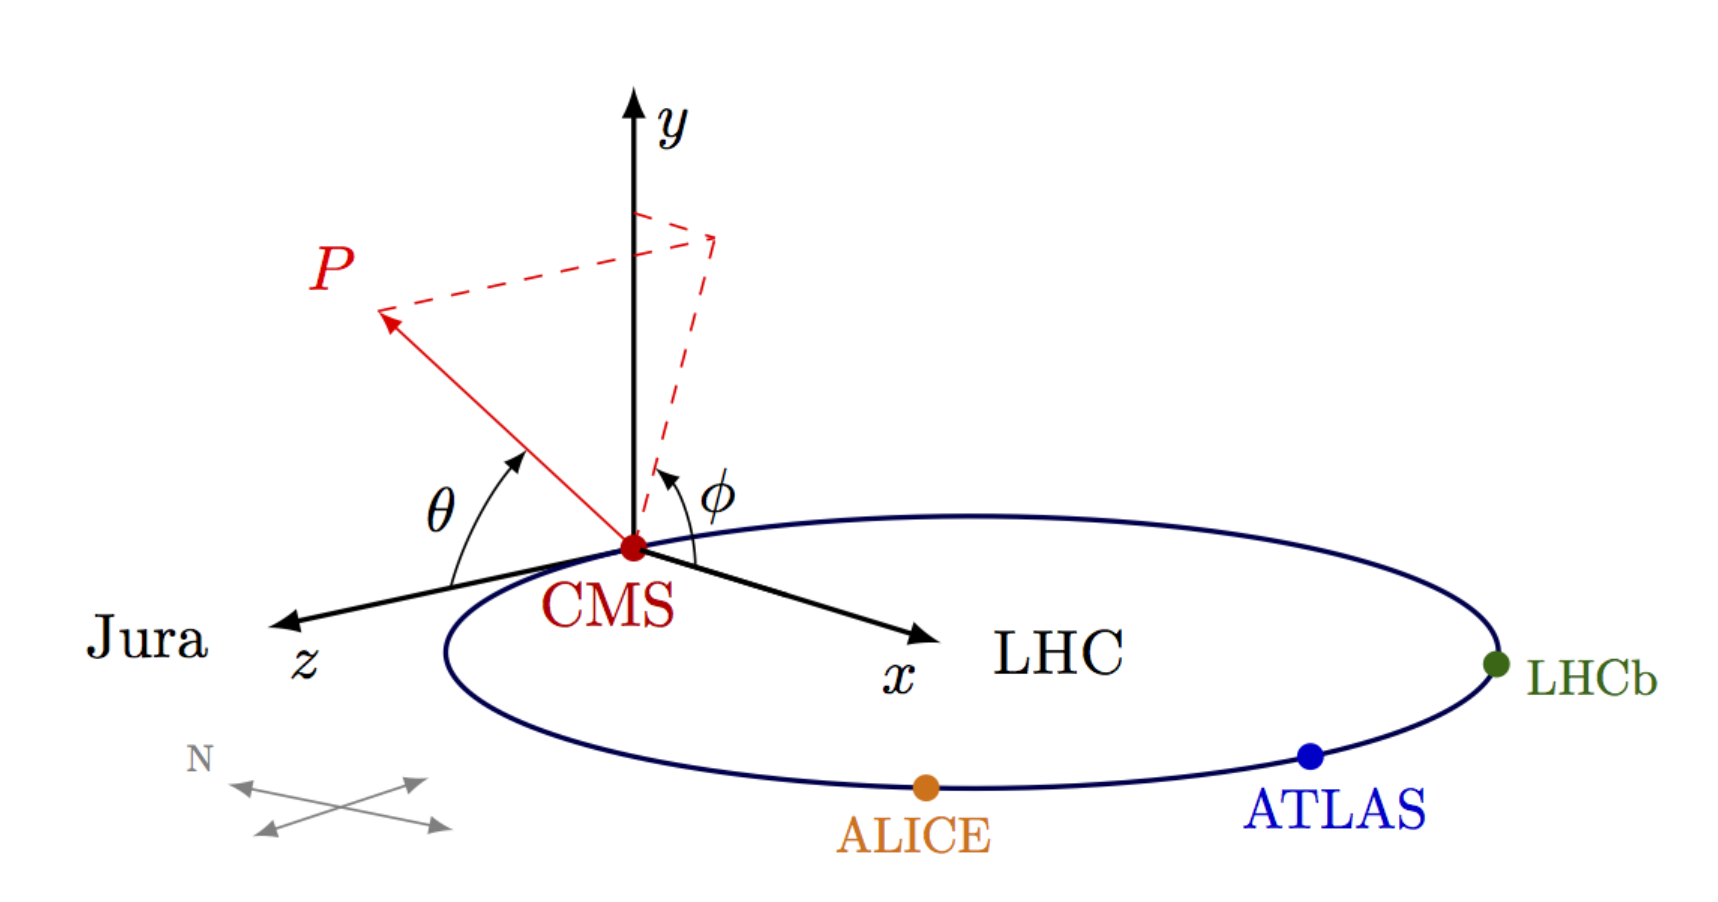
\includegraphics[width=0.9\textwidth]{figures/02-CMS/cms/coordinate.png}
    \caption{The conventional CMS coordinate system.}
    \label{fig:02_cms_coords}
\end{figure}

\section{Detecting particles}
\label{sec:02_cms_particles}

\subsection{Particle interactions with matter}
\label{sec:02_cms_interactions}

In Part~\ref{part:sm}, we discussed the interpretation of fundamental particles as irreps of the Poincar\'e group and quantum excitations of fields.
In experimental physics, we have yet another interpretation: ``a particle is an object that interacts with your detector such that you can follow its track'' (W. Riegler~\cite{Riegler2013}).

Which is to say, in order to detect particles, they must interact with the detector material and transfer energy in a way that we can measure.
Out of the myriad particles produced in LHC proton-proton collisions, the are only eight particles stable enough to reach the CMS detector and be detected are listed in Table~\ref{tab:02_cms_particles}.
% are only nine particles stable enough to reach the CMS detector: photons, protons, neutrons, electrons, muons, charged pions, charged kaons, neutral kaons, and neutrinos.
Neutrinos are also stable, but are too weakly interacting to measure with the CMS detector, which means it is vital to measure the energy of all the other particles hermetically; the presence of neutrinos can then be inferred by energy conservation, or ``missing energy'' carried by neutrinos.

\begin{table}[ht!]
    \centering
    % \captionsetup{justification=centering}
    \caption{Particles which can reach and be detected by the CMS detector. Lifetimes are given in the rest frame for unstable particles.}
    \label{tab:02_cms_particles}
    \begin{tabular}{@{}lccc@{}}
        \toprule
        \textbf{Particle} & \textbf{Mass (MeV/$c^2$)} & \textbf{Charge ($e$)} & \textbf{Lifetime (s)} \\
        \midrule
        Photons                      & $0$                    & $0$     & Stable \\
        Electrons / positrons         & $0.511$                & $\pm1$    & Stable \\
        Protons                      & $938$                  & $+1$    & Stable \\
        Neutrons                    & $940$                 & $0$     & $880$ \\
        (Anti-)Muons                       & $106$                  & $\pm1$    & $2.2 \times 10^{-6}$ \\
        Charged pions                & $140$                  & $\pm1$  & $2.6 \times 10^{-8}$ \\
        Neutral kaons               & $498$                 & $0$                     & $9 \times 10^{-11}$---$5 \times 10^{-8}$ \\
        Charged kaons                & $494$                  & $\pm1$  & $1.2 \times 10^{-8}$ \\
        \cbottomrule
    \end{tabular}
\end{table}

\subsubsection{Charged particles}

Out of these eight, the charged particles can interact electromagnetically with matter through:
\begin{itemize}
    \item Ionization and excitation of atoms: inelastic scattering with atomic electrons and elastic scattering from nuclei, respectively.
    The average energy loss per distance $\left\langle \cnicefrac{dE}{dx}\right\rangle$ of a particle due to ionization is given by the famous Bethe-Bloch formula~\cite{bethe1953passage}.
    \item Bremsstrahlung: photon radiation because of (de-)acceleration in the electric field of nuclei;
    \item Cherenkov effect: photon radiation due to the particle moving faster than the speed of light in the medium;
    \item and transition radiation: photon radiation due to the crossing a boundary between two different dielectrics.
\end{itemize}
Generally, for ``heavy'' charged particles (of mass $\gg$ electron mass), electromagnetic interactions are dominated by ionization and excitation, while for electrons and positrons, Bremsstrahlung is dominant at higher energies.
% The trajectories of low energy electrons and positrons can also deviate significantly due to \textit{multiple scattering} in the material.

The presence and angle of Cherenkov radiation depends on the particle momenta, a fact which is often exploited for ``particle identification'' (PID) by distinguishing particles of different masses at given momenta.
For example, LHCb uses ring-imaging Cherenkov (RICH) detectors to distinguish hadrons, which is critical for $b$-physics~\cite{LHCb:2008vvz}.
CMS, on the other hand, did not prioritize PID and cannot accurately distinguish between the different hadrons beyond their charge.

% accurately distinguish only between charged and neutral hadrons.

\subsubsection{Photons}

Photons primarily interact through:
\begin{itemize}
    \item The photoelectric effect: absorption by an atom causing the ejection of an electron, dominant at low energies, $\ll 1\MeV$;
    \item Compton scattering: incoherent scattering off an atomic electron, dominant at intermediate energies, $\sim 1\MeV$;
    \item and pair production: converting into electron-positron pairs in the Coulomb field of nuclei, dominant at high energies, $\gg 1\MeV$.
\end{itemize}
The combination of these effects means that as high energy electrons and photons propagate through the detector material, they produce a cascade of secondary particles, called an \textit{electromagnetic shower}, which are analyzed to infer the presence and overall energy of the originating particle.

It is often convenient to characterize detector materials by their \textit{radiation length} ($X_0$), which is the mean distance into the material over which high-energy electrons lose $\cnicefrac{1}{e}$ of their energy due to Bremsstrahlung, and $\cnicefrac{7}{9}$ of the mean free path of photons before pair production.

\subsubsection{Hadrons}

Finally, high energy hadrons can also interact with atomic nuclei through the strong force, losing energy through further particle emissions which create their own \textit{hadronic shower}.
As a large fraction of these emitted particles are neutral pions, which decay immediately into photons, hadronic showers are also often accompanied by electromagnetic sub-showers.
We can characterize materials for hadron detection similarly by their \textit{nuclear interaction length} ($\lambda$), the mean free path between nuclear interactions.

\subsection{Types of detectors}
\label{sec:02_cms_detecting_detectors}

\subsubsection{Tracking detectors}

The earliest particle detectors were gaseous \textit{ionization chambers}.
Charged particles passing through these detectors ionize the gas along their trajectory, creating visible tracks, which can be captured, for example, by using an electric field to push the ions towards photographic film.
The most notable examples are cloud chambers, which were prominent in the first half of the 20th century, and led to the discovery of the positron, muon, and kaon via cosmic rays.
The Nobel Prize was awarded to Charles Wilson in 1927 and Carl Anderson in 1936 for the invention and development of the cloud chamber, respectively.

% for the invention of the cloud chamber, and to Carl Anderson in 1936 for the discovery of the positron.
% Charles Wilson and Carl Anderson were awarded the Nobel Prize in 1927.
% as well as Nobel prizes for their inventors.

Tracking detectors have since continuously evolved, such as through the use of liquid media in \textit{bubble chambers} and charged wires to produce electric fields and read out ionization signals electronically in \textit{wire chambers}, both of which again led to Nobel Prizes for their inventors, Donald Glaser and Georges Charpak, respectively.
% Both inventions again led to Nobel Prizes, for Donald Glaser in 1960 and Georges Charpak in 1992, respectively.
The Gargamelle bubble chamber at CERN notably led to the discovery of weak neutral currents~\cite{GargamelleNeutrino:1973jyy} (see Chapter~\ref{sec:01_sm_ew_weak}).

More recently, a significant advancement in tracking detectors has been achieved through the use of semiconductors such as silicon.
A $p$-$n$ semiconductor diode~\cite{sparkes1994semiconductor, Nomerotski:2009zz} effectively forms an ionization chamber as well, where charged particles passing through will create electron-hole pairs whose charge can be collected and recorded.
Semiconductor detectors can have lower ionization energies, higher granularity, better position and time resolution, and strong radiation tolerance, while also being able to leverage innovations and state-of-the-art fabrication techniques from the semiconductor industry.

Thus, there has been a gradual shift towards their use, particularly in collider physics.
Here, tracking detectors are crucial for (1) \textit{vertexing} --- measuring particle tracks precisely to determine the point of collision, or the ``vertex'' --- and (2) measuring the curvature of charged-particle trajectories in a magnetic field to determine their momenta.
Silicon trackers, for example, were employed for vertexing in all LEP experiments and the CDF and D\O experiments at the Tevatron.
The CMS detector is notably the first to use silicon for its entire tracking volume.

Semiconductor trackers are, however, more expensive per unit area.
Hence, gaseous and liquid detectors remain prevalent in particle physics, particularly where large volumes are required, such as in neutrino experiments and the CMS muon system.

\subsubsection{Calorimeters}

Calorimeters are detectors designed primarily to measure the energy of particles.
They can be either \textit{homogeneous}, where the entire volume of the detector can both absorb \textit{and} measure the energy of the shower; or, \textit{sampling}, where separate ``passive'' layers which absorb energy and initiate the shower are interleaved with ``active'' layers to measure the energy.
Sampling calorimeters are less precise than homogeneous calorimeters, but are more cost-effective, especially when large volumes are required.
CMS employs both types of calorimeters, and primarily uses \textit{scintillation} --- photon emission due to atomic (de-)excitation from charged particles --- to capture and measure energy.

Generally in collider physics trackers are designed to have short radiation lengths, to minimize particle energy loss, and calorimeters as long a radiation length as possible, to capture the entire energy of electromagnetic or hadronic showers.
In addition to their radiation and nuclear interaction lengths, calorimeter materials are characterized as well by their \textit{Moli\`ere radius} ($R_M$), which is the radius of a cylinder containing, on average, 90\% of an incident electron or photon's electromagnetic shower energy.
It is approximately related to $X_0$ as:
\begin{equation}
    \label{eq:02_cms_moliere}
    R_M = 0.0265 X_0 (Z + 1.2),
\end{equation}
where $Z$ is the atomic number of the material.

\subsubsection{General-purpose detectors}

Designing a general-purpose detector, such as CMS, requires a careful optimization of several factors, including high efficiency and resolution for as many of the particles in Table~\ref{tab:02_cms_particles}, radiation hardness, cost effectiveness, and more.
A typical compromise in particle physics has been a ``layered'' detector design, as shown in Figure~\ref{fig:02_cms_layers}, with a thin (in radiation and nuclear interaction lengths) innermost tracker for precise vertexing and momentum measurements, followed by thick calorimeters to measure particle energies, and finally dedicated detectors to identify and measure high energy muons that are able to penetrate the previous layers.
The CMS detector follows this general philosophy, as shown in Figure~\ref{fig:02_cms_slice}.

\begin{figure}[ht]
    \centering
    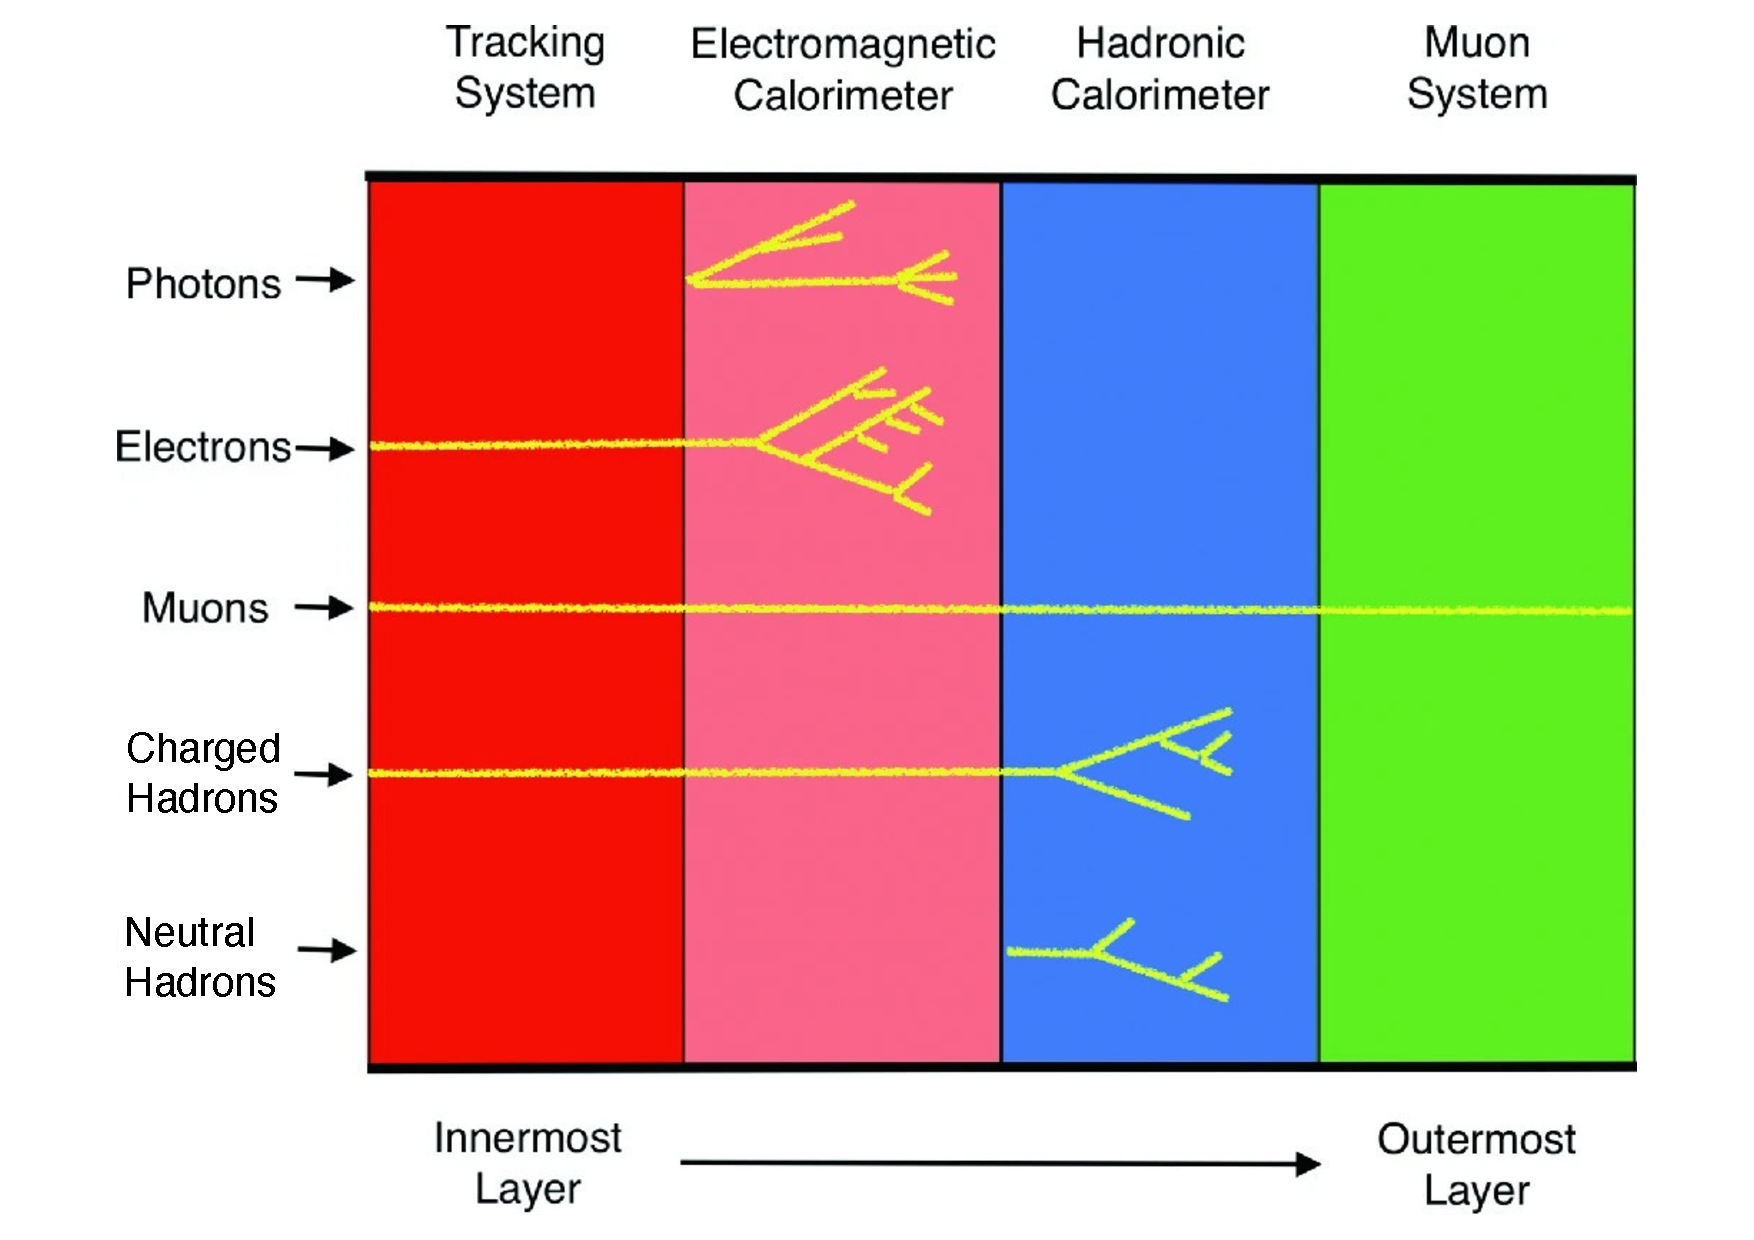
\includegraphics[width=\textwidth]{figures/02-CMS/cms/interactions_layers_edit2.pdf}
    \caption{Layers in a typical general-purpose detector in particle physics and an illustration of the interactions of different particles.}
    \label{fig:02_cms_layers}
\end{figure}

\begin{figure}[ht!]
    \centering
    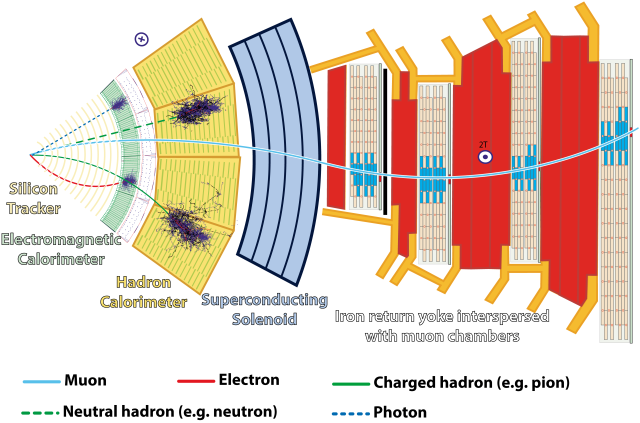
\includegraphics[width=\textwidth]{figures/02-CMS/cms/components/slice.png}
    \caption{Illustration of the different detector layers in the CMS barrel region and the expected hits and energy deposits from various particles, reproduced from Ref.~\cite{Davis:2205172}.}
    \label{fig:02_cms_slice}
\end{figure}

\section{CMS detector components}
\label{sec:02_cms_detectors}

\subsection{The magnet}
\label{sec:02_cms_magnet}

The defining characteristic of the CMS detector is its strong $3.8\unit{T}$ solenoid magnet, with a $11.4 \unit{T\,m}$ bending power (Figure~\ref{fig:02_cms_magnet}).
% , which allows precise measurements of charged-particle momenta in the tracker.
Its large $6\unit{m}$ diameter and $13\unit{m}$ length accommodate not only the tracker for momentum measurements, but also the calorimeters in order to reduce the material in front of them.
The strength of the magnet was chosen to allow precision measurements of charged-particle momenta and to achieve a target \pt resolution of 10\% for 1\TeV muons.

\begin{figure}[ht]
    \centering
    \includegraphics[width=\textwidth]{figures/02-CMS/cms/components/magnet_lowering.jpg}
    \caption{The CMS solenoid, as it was being lowered into the CMS cavern in 2007, reproduced from Ref.~\cite{Maximilien:1020310}.}
    \label{fig:02_cms_magnet}
\end{figure}

As shown in Figures~\ref{fig:02_cms_detector} and~\ref{fig:02_cms_slice} in red, the solenoid is additionally surrounded by massive layers of steel ``return yoke'', weighing 12,000 tonnes in total, for several complementary reasons:
(1) it confines the magnetic field, improving the efficiency and safety of the detector, by providing a low-reluctance path for the magnetic field lines to return to the solenoid;
(2) it is interleaved with the CMS muon system and provides a residual magnetic field for muon tracking;
(3) it absorbs the remaining particles not been completely contained by the calorimeters;
and, finally, (4) it provides structural support to the detector.
The resulting magnetic field throughout CMS is shown in Figure~\ref{fig:02_cms_magnetic_field}, where we can see a uniform $3.8\unit{T}$ field within the solenoid and an $\approx 2\unit{T}$ field in the return yoke.

\begin{figure}[ht]
    \centering
    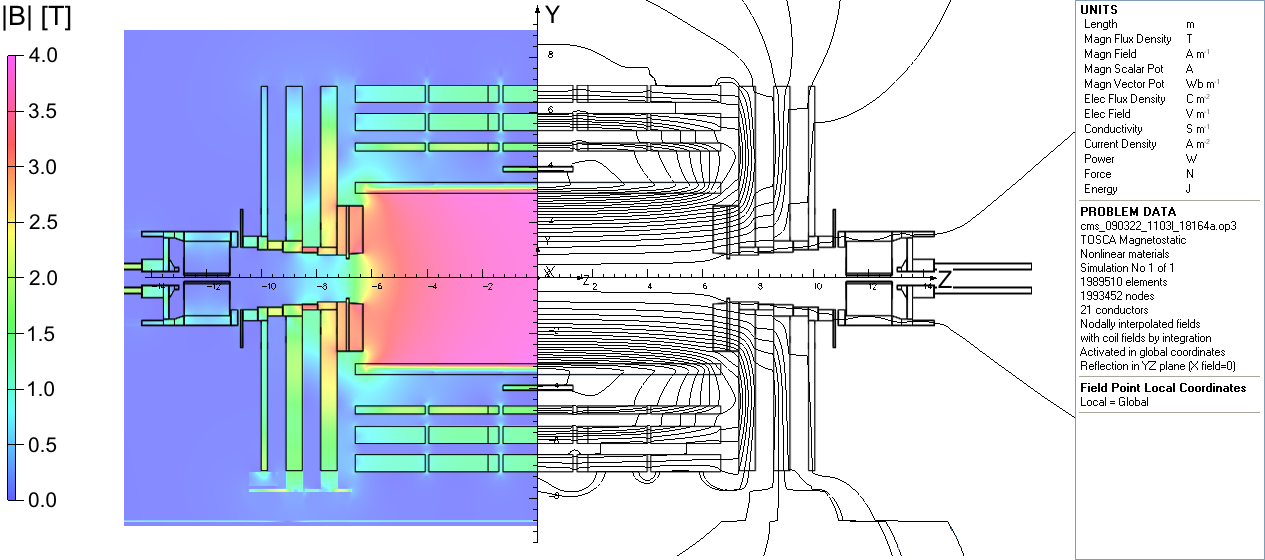
\includegraphics[width=\textwidth]{figures/02-CMS/cms/components/magnetic_field}
    \caption{Measurement using cosmic rays (left) and illustration (right) of the CMS magnetic field, reproduced from Ref.~\cite{CMS:2009moq}.}
    \label{fig:02_cms_magnetic_field}
\end{figure}

\subsection{Tracker}
\label{sec:02_cms_tracker}

\begin{figure}[ht]
    \centering
    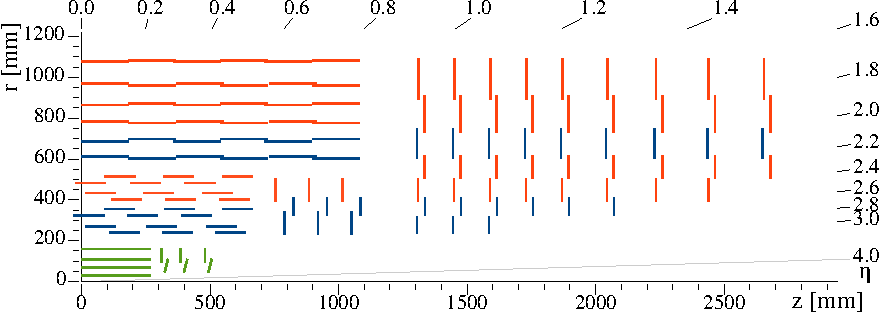
\includegraphics[width=\textwidth]{figures/02-CMS/cms/components/Phase1_Tracker_1Quarter.pdf}
    \caption{Schematic of one quarter of the Phase-1 CMS tracker in the $r$-$z$ plane, reproduced from Ref.~\cite{CMS:2017lum}.
    In green are the pixel detector layers, in red the single-sided strip modules, and in blue the double-sided strip modules.}
    \label{fig:02_cms_tracker}
\end{figure}

The CMS tracker is designed to achieve the key detector requirements of strong charged-particle momentum resolution and efficient online and offline $\tau$ and $b$-jet reconstruction.
It must additionally operate at a high efficiency at the expected average pileup rate of 20-60 collisions per bunch crossing in Runs 1--3 of the LHC.
To do so, as illustrated in Figure~\ref{fig:02_cms_tracker}, it comprises relatively small and granular silicon \textit{pixel} layers close to the interaction point for precise vertexing, followed by larger silicon \textit{strip} layers.
The tracker has an overall diameter of 2.5m and length of 5.8m, and is composed of a separate co-axial ``barrel'' region and two ``endcap'' regions perpendicular to the beamline, to provide pseudorapidity coverage of $\abs{\eta} \lesssim 2.4$.

Silicon has several advantages for tracking detectors: it can be made radiation hard to be placed close to the interaction point~\cite{BaselgaBacardit:2015iqn}; it has a low ionization energy of $3.6$\unit{eV}; it can be made thin --- the maximum radiation and nuclear interaction lengths over the entire CMS tracker are around $2$ and $0.6$ respectively (Figure~\ref{fig:02_cms_tracker_material}); it is naturally abundant and widely used in the semiconductor industry; and it can be easily patterned to small dimensions for high granularity.
This is why, as discussed in Section~\ref{sec:02_cms_detectors}, silicon has gained popularity in particle physics, with CMS being the first to use it for the entire tracker.
% Because of these benefits, silicon has gradually gained prominence for particle tracking, being employed for vertexing in all LEP experiments and the CDF and D0 experiments at the Tevatron.
% The CMS detector was the first to use silicon for the entire tracker.

\begin{figure}
    \centering
    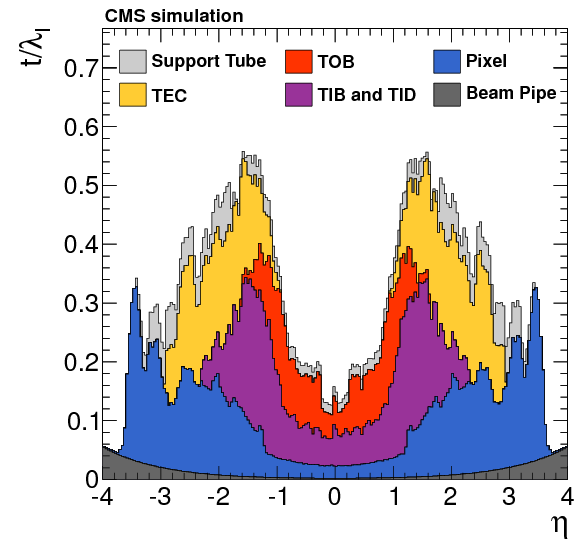
\includegraphics[width=0.49\textwidth]{figures/02-CMS/cms/components/figs_2011_cmsTracker_MaterialBudget_InteractionLengths.png}
    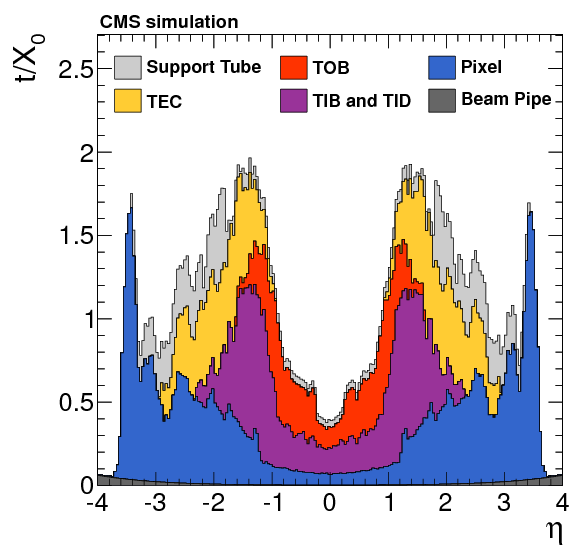
\includegraphics[width=0.49\textwidth]{figures/02-CMS/cms/components/figs_2011_cmsTracker_MaterialBudget_RadLengths.png}
    \caption[Total thickness $t$ of the tracker material traversed by a particle produced at the nominal interaction point.]{Total thickness $t$ of the tracker material traversed by a particle produced at the nominal interaction point, as a function of pseudorapidity $\eta$, expressed in units of radiation length $X_0$ (left) and nuclear interaction length $\lambda_I$ (right), reproduced from Ref.~\cite{CMS:2014pgm}.}
    \label{fig:02_cms_tracker_material}
\end{figure}

The pixel tracker includes three barrel layers at radii of 4.4, 7.3, and 10.2\unit{cm} and two pairs of endcap disks at $z = \pm34.5$ and $\pm46.5\unit{cm}$.
It contains a total of 1440 modules and 66 million pixels, of size (or ``pitch'') $100\times150$\unit{$\mu$m$^2$}, and thickness $285$\unit{$\mu$m}.
The planar position of the sensor provides a third position coordinate as well.
The pixel tracker yields an overall hit position resolution of $10$--$20$\unit{$\mu$m} in the transverse direction --- $r\phi$ in the barrel ---  and $20$--$40$\unit{$\mu$m} in the longitudinal direction --- $z$ in the barrel.
The pixel orientation is optimized most for $r\phi$ resolution, as that is the plane in which charged particles bend from the CMS magnetic field.

Silicon strip modules are longer than pixels, providing high granularity only in one axis, but are more cost-effective; hence, they are used in the outer layers of the CMS tracker, which require a much larger area of coverage: $198$\unit{m$^2$} of active coverage versus $1.1$\unit{m$^2$} for the pixels.
The strip tracker has 10 barrel layers and three small and nine large endcap disks, with a total of 15,148 modules and 9.3 million strips.
It contains two types of strip modules: standard ``single-sided'' modules as well as ``double-sided`` modules mounted back-to-back at a stereo angle to effectively allow pixel-like 2D measurements as well, albeit at a lower granularity.

The strip modules in the barrel are aligned parallel to the beamline with a pitch ranging from $80$--$183$\unit{$\mu$m}, while those in the endcaps are mounted in the radial direction with a pitch of $81$--$205$\unit{$\mu$m}.
Overall, the strips in the inner barrel and disk layers provide an $r\phi$ resolution of $13$--$38$\unit{$\mu$m}, while the outer layers provide $18$--$47$\unit{$\mu$m}.


\subsection{ECAL}

The CMS electromagnetic calorimeter (ECAL) (Figure~\ref{fig:02_cms_ecal}) was designed to precisely measure energies of electrons and photons.
It was particularly optimized for sensitivity to the Higgs-to-two-photon decay channel, which proved crucial to the discovery of the Higgs boson~\cite{CMS:2012qbp}.
% It was especially optimized for high sensitivity to the Higgs to two photon decay channel, which proved crucial to the discovery of the Higgs boson.

The ECAL is a homogeneous calorimeter made out of 75,848 lead-tungstate (PbWO$_4$) crystals (Figure~\ref{fig:02_cms_ecal_crystals}), which are a type of highly transparent scintillators.
PbWO$_4$ was chosen for its high density (8.28\unit{g/cm$^3$}), short radiation length ($X_0 = 0.89\unit{cm}$), and small Moli\`ere radius ($R_M = 2.2\unit{cm}$), which allows for a compact calorimeter with fine granularity.
Additionally, its fast scintillation response ($\approx 10\unit{ns}$) allows distinguishing between ``out-of-time'' (OOT) pileup --- particles produced from adjacent bunch crossings --- and particles from the primary interaction~\cite{CMS:2020xlg}.
%  and the ability to minimize ambiguity between particles from different bunch crossings.
The scintillation light is detected by photodiodes glued to the back of each crystal.

\begin{figure}[ht]
    \centering
    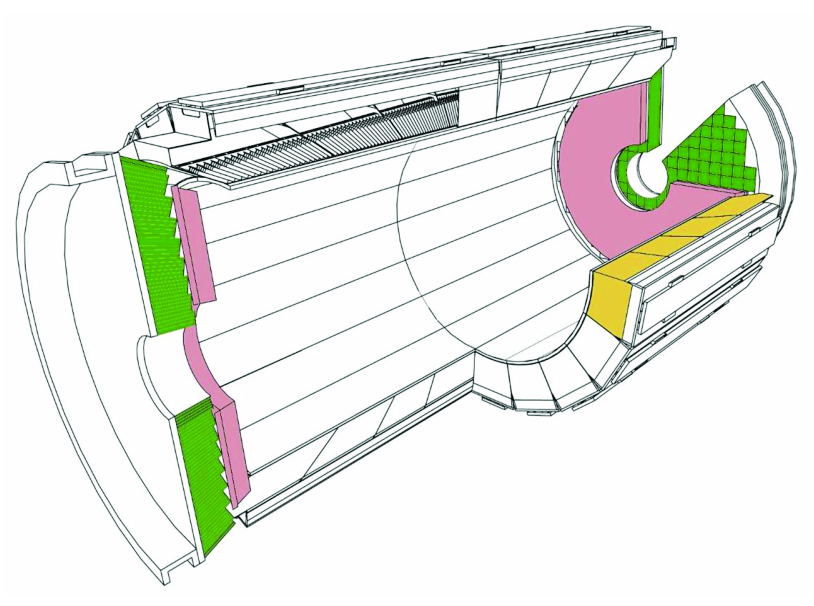
\includegraphics[width=\textwidth]{figures/02-CMS/cms/components/ecal_layout.png}
    \caption{Layout of the CMS ECAL, reproduced from Ref.~\cite{Cooke:2022lbl}, with one of the 36 barrel regions highlighted in yellow, the preshower in pink, and the endcap regions in green.}
    \label{fig:02_cms_ecal}
\end{figure}

\begin{figure}[ht]
    \centering
    \captionsetup{justification=centering}
    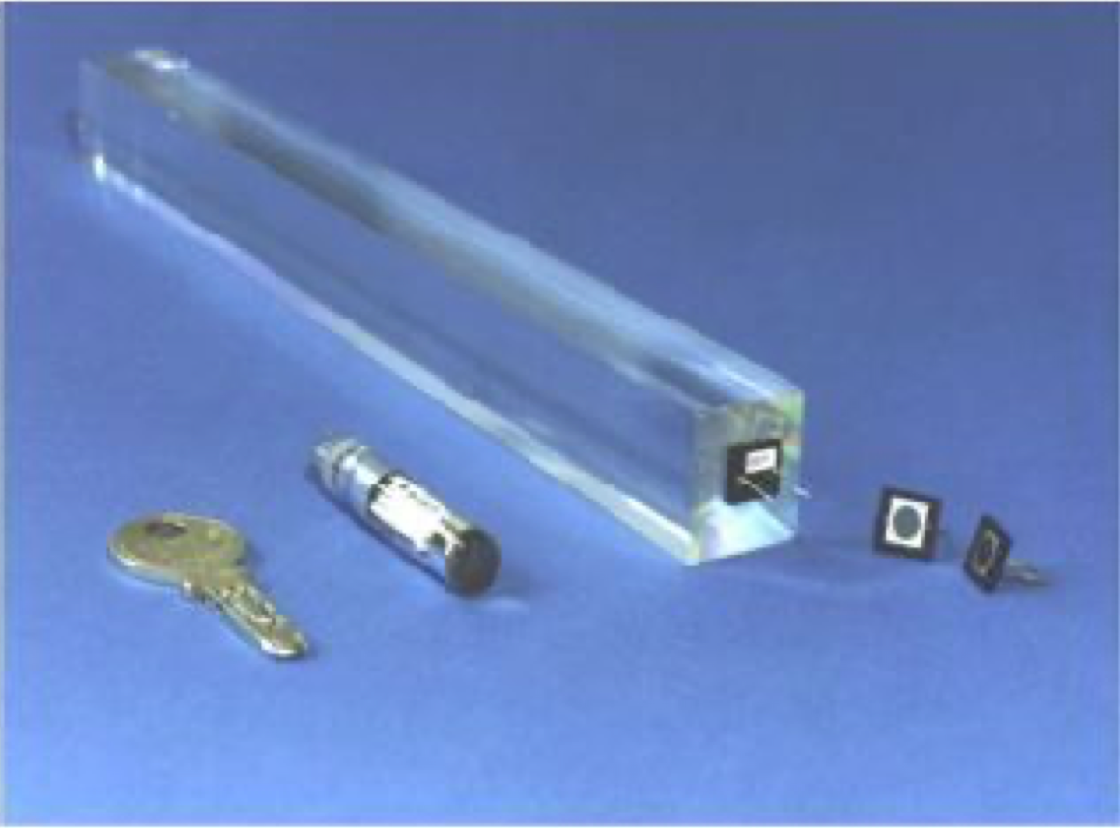
\includegraphics[width=0.4\textwidth]{figures/02-CMS/cms/components/PbWO4_crystals.png}
    \caption{PbWO$_4$ crystals and photodiodes used in the CMS ECAL.}
    \label{fig:02_cms_ecal_crystals}
\end{figure}

Like the tracker, it has a barrel region, covering $\abs{\eta} < 1.48$, and two endcap regions for $1.48 < \abs{\eta} < 3.00$.
They have thicknesses of $25.8X_0$ and $24.7X_0$, respectively, and a total nuclear interaction length of around 1.
This is sufficient to contain >$98\%$ of the energy of $\leq 1\TeV$ electrons and photons, and causes around two thirds of charged hadrons to shower in the ECAL as well.

Additionally, the ECAL includes a ``Preshower'' sampling calorimeter in the endcap regions, which comprises two layers of $3X_0$ of lead to initiate electromagnetic showers, interleaved with active silicon strip detectors for measurements.
The purpose of the Preshower is primarily to distinguish between single photons and neutral pion decays into two, close-by, photons in the forward regions, whose energy deposits in the ECAL would otherwise overlap significantly.

\subsection{HCAL}

The CMS hadronic calorimeter (HCAL) sits roughly $30\unit{cm}$ outside the ECAL and is designed to measure the energies of neutral and charged hadrons.
It is composed of four major sections: the HCAL barrel (HB), the HCAL endcap (HE), the HCAL outer (HO), and the HCAL forward (HF) (Figure~\ref{fig:02_cms_hcal}).
Due to their much greater volume compared to the ECAL, the HB, HE, and HO are all chosen to be sampling calorimeters, with alternating layers of absorber material and plastic scintillator.
The HF extends the pseudorapidity coverage of CMS up to $\abs{\eta} = 5.2$ and is a steel and quartz-fiber \textit{Cherenkov calorimeter}.

The HB has 14 total layers of brass absorbers and scintillators, with additional steel front and back plates, covering $\abs{\eta} < 1.4$~\cite{CMS:2008xjf}.
Due to its radial constraints, with the ECAL and magnet on either side, it has a thickness at $\eta = 0$ of only $5.8\lambda$, with the ECAL adding another $\approx1\lambda$.

\begin{figure}[ht]
    \centering
    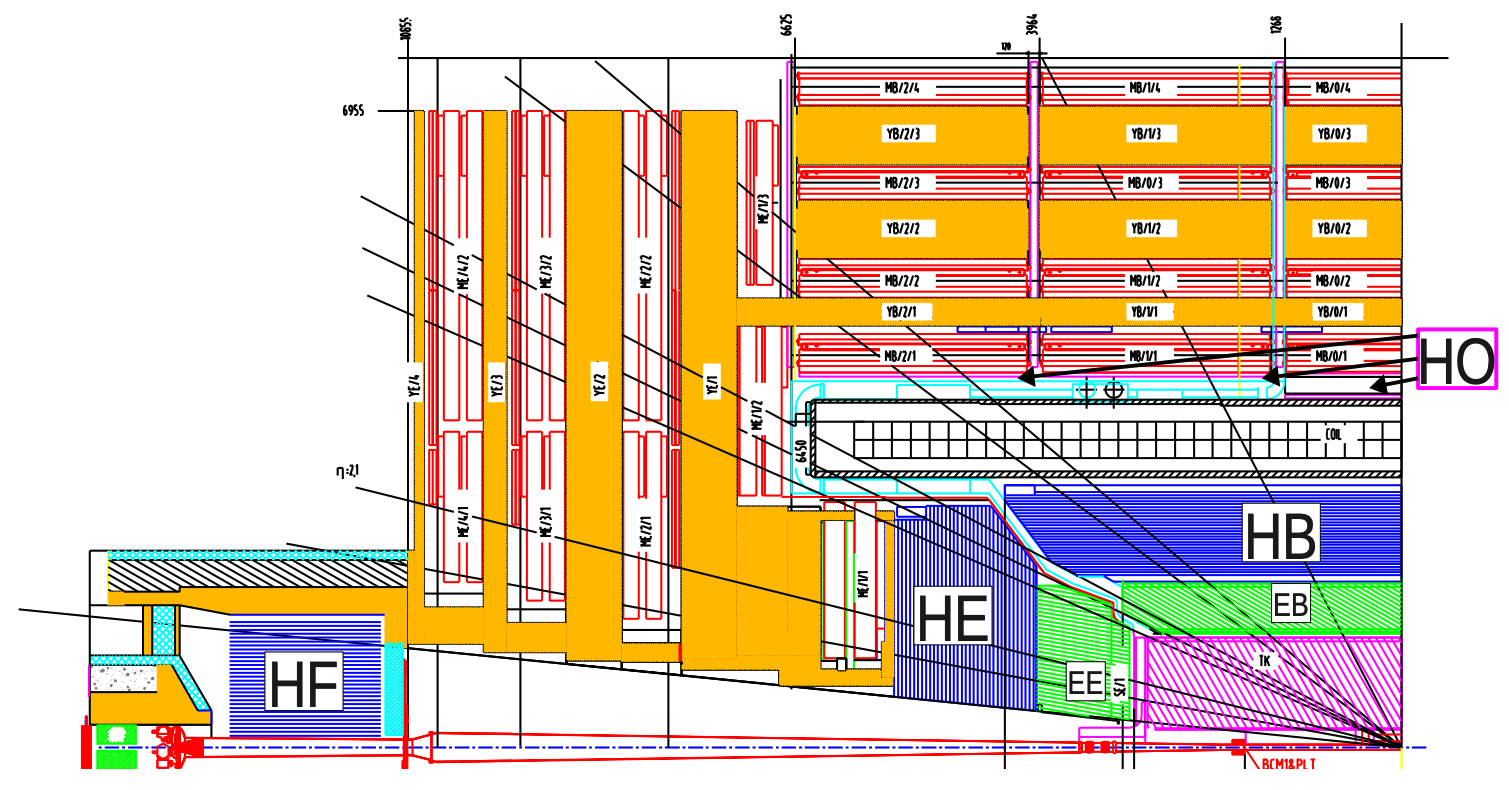
\includegraphics[width=\textwidth]{figures/02-CMS/cms/components/hcal_layout.png}
    \caption{Layout of the CMS detector in the $r$-$z$ plane with the four HCAL sections labeled, reproduced from Ref.~\cite{CMS:2012tda}.}
    \label{fig:02_cms_hcal}
\end{figure}

To capture the remaining ``tails'' of hadronic showers in the barrel region, the HO is placed outside the solenoid.
It uses the same scintillators and electronics as the HB, but uses the magnet and return yoke materials themselves as absorbers, adding up to $3\lambda$ more of material.
Figure~\ref{fig:02_cms_hcal_ho} demonstrates that the HO is crucial for capturing the entire energy of hadronic showers: without it, we see an excess of events with the measured energy of hadrons lower than their incident energy, implying a loss of energy with the HB alone.

\begin{figure}[ht]
    \centering
    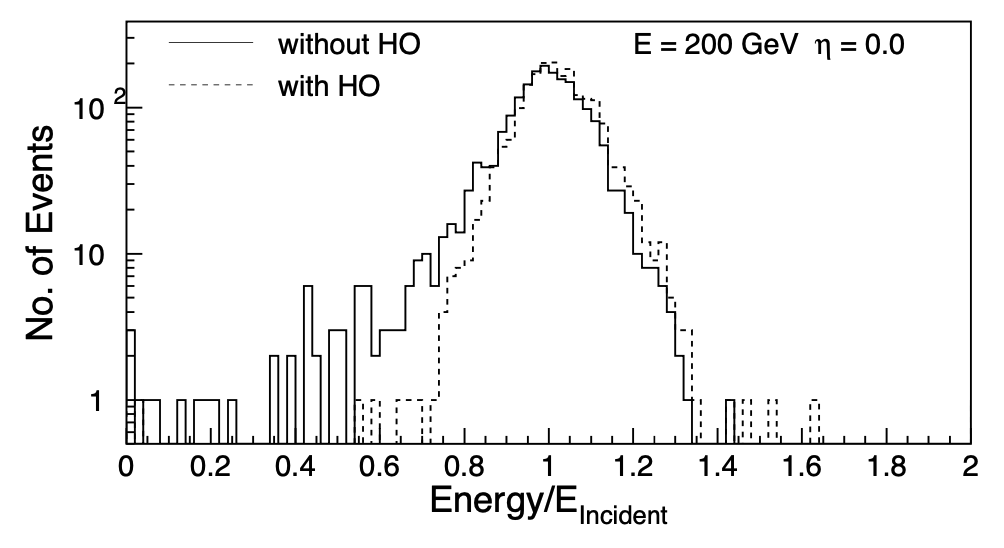
\includegraphics[width=0.7\textwidth]{figures/02-CMS/cms/components/hcal_ho_energy.png}
    \caption[Simulation of the distribution of measured $/$ incident energy for pions with incident energies of $200\GeV$ at $\eta = 0$, reproduced from Ref.~\cite{CMS:2008xjf}.]{Simulation of the distribution of measured $/$ incident energy for pions with incident energies of $200\GeV$ at $\eta = 0$, reproduced from Ref.~\cite{CMS:2008xjf}.
    Without the HO, there is an excess of events with the measured energy lower than the incident, while with the HO the distribution is a Gaussian centered at 1, implying recovery of the total pion shower energy.}
    \label{fig:02_cms_hcal_ho}
\end{figure}

The HE covers the pseudorapidity range $1.3 < \abs{\eta} < 3.0$ and has 18 layers of brass and scintillators, for a total length of $10\lambda$ including the ECAL.
The granularity of both the HB and HE for $\abs{\eta} < 1.6$ is $0.087\times0.087$ in $\eta$-$\phi$, while for $\abs{\eta} > 1.6$ in the HE it increases to $0.17\times0.17$.

The HF is placed 11.2\unit{m} from the interaction point to cover the very forward range $3.0 < \abs{\eta} < 5.2$.
Its primary design constraints are the extremely hostile radiation levels in the high-rapidity region, and hence uses steel absorbers and quartz fibers that are radiation hard~\cite{Penzo:2009zz}.
It contains $1.65\unit{m}$ of absorber material in each endcap, and measures energy through Cherenkov light emitted by charged particles moving through the longitudinal quartz fibers.
It is hence more sensitive to the electromagnetic component of showers.

The HF is important in measuring the energy of an event hermetically and, thereby, the missing energy as well.
Moreover, it is crucial in identifying highly forward jets like those produced through VBF-production of Higgs bosons, an important production-mode measured in this dissertation (see Chapters~\ref{sec:01_higgs} and~\ref{sec:05_hh}).


\subsection{Muon system}

As implied by its name, detecting muons with high efficiency and precision was a key consideration in the design of CMS.
This is because of their unique signature compared to the other particles in Table~\ref{tab:02_cms_particles}, the possibility of Higgs discovery in the $H\to ZZ^*\to 4\mu$ channel, and the relatively low isolated-muon background at the LHC.
Indeed, the $4\mu$ channel was crucial to the discovery of the Higgs boson~\cite{CMS:2012qbp}.

Muons are detected through a combination of the silicon tracker inside the solenoid, and dedicated gas ionization chambers for tracking muons outside the solenoid, covering a total pseudorapidity range of $\abs{\eta} < 2.4$.
The muon system, being the outermost subdetector, needs to cover the largest amount of area --- around 25,000m$^2$ of detector layers --- and hence uses gaseous detectors to minimize cost while maintaining reliability and robustness.
Three types of gas detectors are used: drift tubes (DTs) in the barrel region, cathode strip chambers (CSCs) in the endcap regions, and resistive plate chambers (RPCs) in both, all housed between the steel flux return yoke layers, as shown in Figure~\ref{fig:02_cms_muon}.

\begin{figure}[ht]
    \centering
    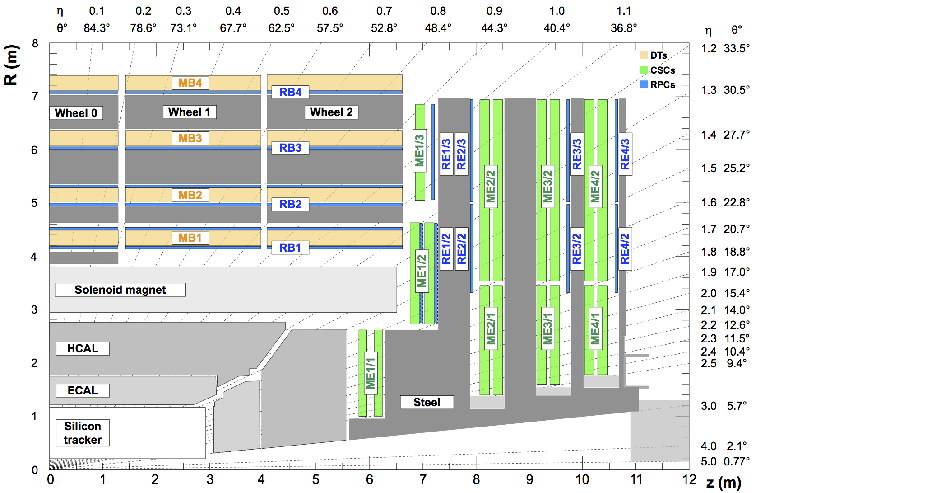
\includegraphics[trim=0pt 0pt 90pt 0pt, width=\textwidth]{figures/02-CMS/cms/components/muon_system}
    \caption[Layout of the CMS detector in the $r$-$z$ plane, with the muon system highlighted and the steel return yoke in dark grey, reproduced from Ref.~\cite{CMS:2018rym}.]{Layout of the CMS detector in the $r$-$z$ plane, with the muon system highlighted and the steel return yoke in dark grey, reproduced from Ref.~\cite{CMS:2018rym}.
    The drift tube stations (DTs) are labeled MB (“Muon Barrel”) and the cathode strip chambers (CSCs) are labeled ME (“Muon Endcap”).
    Resistive plate chambers (RPCs) are mounted in both the barrel and endcaps of CMS, where they are labeled RB and RE, respectively.
    }
    \label{fig:02_cms_muon}
\end{figure}

Because of the lower radiation and background levels expected in the barrel region, standard DT chambers are used, which are known to have excellent spatial and timing resolution while remaining relatively inexpensive.
There are four muon barrel (MB) radial layers, or ``stations''.
The innermost three each contain eight chambers measuring the position in the $r$-$\phi$ plane and four measuring the $z$ coordinate.
The outermost contains only the $r$-$\phi$ chambers.

Each chamber comprises several layers of long aluminum \textit{drift cells}, which have a transverse area of $42\times13$\unit{mm$^2$} and are filled with a mixture of argon (Ar) and carbon dioxide (CO$_2$) gas.
They contain a single anode wire in the center, and the drift time of the electrons to the wire is used to calculate the muon position.
The average single-cell spatial resolution has been measured to be $170\mum$, with a combined per-chamber resolution of $100\mum$ in $r$-$\phi$~\cite{CMS:2008xjf}.
DT chambers also provide a time resolution on the order of nanoseconds, allowing local, independent triggering on muon \pt.

The endcaps are subject to much higher radiation and hence use the more radiation-hard CSCs, which offer fast response times and fine segmentation as well but are more expensive.
They can also tolerate the non-uniformity of the magnetic field in the endcap regions (see Figure~\ref{fig:02_cms_magnetic_field}).
There are four muon endcap (ME) stations on each side, which are divided into ``rings'' in the $r$-direction, and labeled as ME1/2 for the second ring in the first station and so on.

The endcap muon system contains a total of 468 CSCs: 216 in ME1, 108 in ME2 and ME3 each, and 36 in ME4.
A single CSC is composed of six layers of multi-wire proportional chambers, each containing several anode wires spaced between 2.5--3.2\unit{mm} apart and 80 cathode strips to read out position in the $r$-$\phi$ plane~\cite{CMS:2013vyz}.
The CSCs overall provide a spatial resolution in $r$-$\phi$ of $75\mum$ in ME1/1 and ME1/2 and $150\mum$ elsewhere, with a time resolution of <$5\unit{ns}$~\cite{CMS:2008xjf}.
This means CSCs, like the DTs, independently allow local triggering on muon \pt with good efficiency and background rejection.

Finally, RPCs are included as well in both the barrel and endcap regions to provide complementary triggering capabilities.
RPCs are double-gap chambers operated in \textit{avalanche mode}, which means they primarily offer fast timing information, with around $1.5\unit{ns}$ resolution, but relatively poor spatial resolution~\cite{Hebbeker:2017bix}.
There are four RPC barrel (RB) and three RPC endcap (RE) stations, complementing the DTs and CSCs with faster timing information and allowing the muon \pt trigger threshold to be lowered.


\section{Detector reconstruction and performance}
\label{sec:02_cms_reconstruction}

\subsection{Tracker}

Tracks are reconstructed from the hits in the tracker using an iterative algorithm called the Combinatorial Track Finder (CTF)~\cite{CMS:2014pgm}, based on the Kalman filter~\cite{Fruhwirth:1987fm}.
CTF starts by finding the ``easiest'' tracks (e.g. of high \pt and produced near the interaction region), removes their hits from the search, and then repeats the process until all tracks have been found.
Due to the high computational cost of track reconstruction, this cannot be performed at the L1 trigger and, hence, track information is not used for the L1 trigger decision currently in CMS.
% However, the Phase-2 upgrade of the tracker will include outer tracker modules designed especially for fast detection of high \pt tracks, which can be used by the L1 trigger for the first time~\cite{CMS:2017lum}.

Offline, CMS is able to reconstruct isolated muons of $\pt > 0.9\GeV$ with 100\% efficiency within the tracker acceptance of $\abs{\eta} < 2.4$, with a \pt resolution of up to $2.8\%$ for $\pt \sim 100\GeV$~\cite{CMS:2014pgm}.
The pixel tracker can also achieve a vertex position resolution of $10$--$12$\unit{$\mu$m} in all three spatial dimensions.
$B$-hadrons produced in the $pp$ collisions generally travel on the order of a few millimeters before decaying and, hence, the precise vertexing of the CMS tracker allows for efficient $b$-tagging~\cite{CMS:2016kkf} and even boosted $bb$-tagging~\cite{CMS:2023tlv}, as is crucial for the analysis described in this dissertation.

\subsection{ECAL}

Signals in the ECAL crystals are reconstructed by fitting the signal pulse with template pulse shapes to distinguish OOT pileup, both offline and online~\cite{CMS:2020xlg}.
The individual hits are then clustered to identify electromagnetic showers initiated by the same incident particle, and are further clustered into ``superclusters'' to account for photon conversions and bremsstrahlung losses~\cite{CMS:2020uim}.
Clusters are tested for compatibility with reconstructed tracks from both single electrons and pair-produced electrons by photons, and the combined information is used to identify electrons and photons.
Cluster energies are calibrated based on differences in neutral pion to two-photon decays in data and simulation~\cite{CMS:2017yfk}.

With the PF algorithm, electrons (isolated photons) are identified by the ECAL clusters, the presence (absence) of a corresponding track in the tracker, and a low relative energy deposit in the HCAL along the particle trajectory.
The online triggers use a similar but simplified algorithm with tighter requirements on electron and photon identification.
Offline, multivariate regression algorithms are used to correct the raw measured energy for inefficiencies due to energy loss before or in the ECAL.

Overall, the ECAL has been measured in data collected by CMS to have a reconstruction efficiency of >$95\%$ for $10 < E_{\mathrm{T}} < 500\GeV$, with an uncertainty on the electron and photon energy scale of $0.1\%$ in the barrel and $0.3\%$, in the endcaps~\cite{CMS:2020uim}.
Electron energy resolution was measured to be between $2$--$5\%$ in $Z\to e^+e^-$ decays.

\subsection{HCAL}

The energy of hits in the HCAL is estimated, and OOT PU rejected, by fitting pulse templates to the photodetector signals, both online and offline~\cite{CMS:2023lqq}.
Corrections are applied as well based on measured reduction of the light output of the scintillators due to radiation damage and decrease in the photodetector efficiencies~\cite{CMS:2019hpr}.
As the HCAL is a sampling calorimeter, the measured energy must be scaled to estimate the total energy of the hadronic shower.
This scale factor is nonlinear with the energy of the incident particle, and is estimated through a variety of techniques using simulations and data for the different HCAL components and regions~\cite{CMS:2019hpr}.
The overall energy scale is measured to a precision of <$2\%$ in the HB and HE, and <$3\%$ for the HO and HF.

A similar clustering algorithm to the ECAL's is used in all HCAL subdetectors, with the exception of the HF where a hit in a cell is directly considered a ``cluster'.
As hadrons deposit energy in the ECAL as well, cluster energies in both calorimeters are calibrated together for hadrons, using a sample of neutral kaons~\cite{CMS:2017yfk}.
As for electrons and photons in the ECAL, the PF algorithm is used to identify hadrons based on a higher relative energy deposit in the HCAL versus ECAL, and, for the case of charged hadrons, a matching track in the tracker.

Figure~\ref{fig:02_cms_hcal_response} shows the \textit{response} --- the relative mean difference between the measured and true energy of a particle --- and resolution for single neutral hadron energies in the barrel as a function of the true energy, before and after calibration.
We see that the energy resolution is significantly worse than for charged particles and photons --- >10\% for all energies --- due to the modest resolution of the HCAL compared to the tracker and ECAL.
However, neutral hadrons on average comprise only 10\% of event and jet energies (the rest coming from 65\% charged hadrons and 25\% photons), which means the overall contribution is at the percent level.

\begin{figure}[ht]
    \centering
    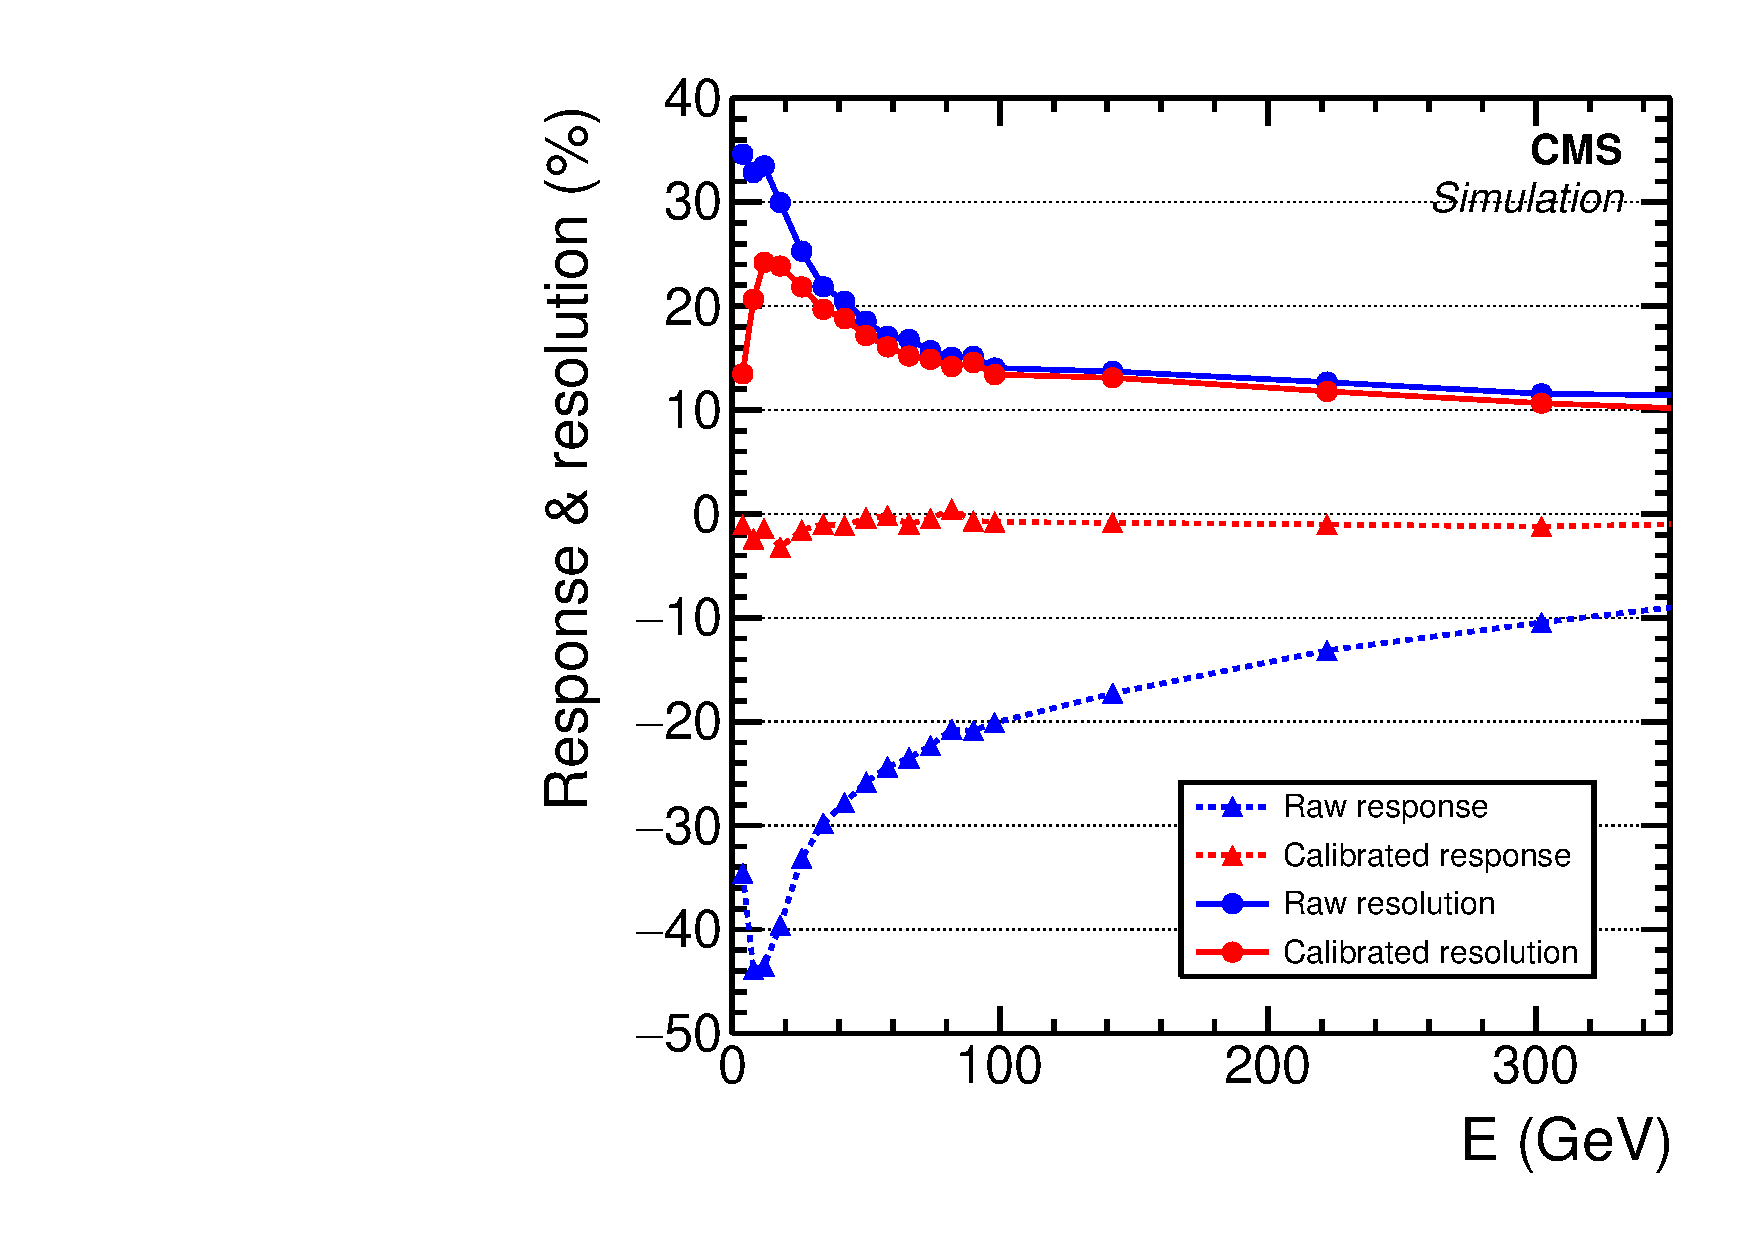
\includegraphics[width=0.7\textwidth]{figures/02-CMS/cms/components/hadron_response.pdf}
    \caption{Response and resolution of single neutral hadron energies in the barrel as a function of the true energy, before and after calibration, reproduced from Ref.~\cite{CMS:2017yfk}.}
    \label{fig:02_cms_hcal_response}
\end{figure}

\subsection{Muon system}

The muon system is triggered using the independent and complementary timing information from the DTs and CSCs in the barrel and endcap, respectively, and the RPCs in both.
% The large number of layers in each muon chamber allows enough \pt precision locally to trigger on muons at the L1
% local triggers
Hits are first reconstructed locally based on the timing information from the RPCs and the position and timing information from the DTs and CSCs.
Hits along the muon chambers are then combined to form \textit{standalone-muon tracks} using a Kalman filter technique~\cite{Fruhwirth:1987fm}.
Additional \textit{tracker muon tracks} and \textit{global muon tracks} are formed by propagating tracker tracks to loosely matched DT or CSC hits, and matching the standalone-muon tracks to tracker tracks, respectively~\cite{CMS:2018rym}.
The combined track information is used by the global PF algorithm to optimize muon identification and determine their momenta~\cite{CMS:2017yfk}.

Overall, the muon reconstruction and identification efficiency has been measured to be >$96\%$~\cite{CMS:2018rym}.
For lower \pt muons ($\pt < 200\GeV$), the momentum measurement is dominated by the inner tracker performance, with a resolution of approximately $1\%$ in the barrel and $3\%$ in the endcaps.
For higher \pt muons, the combined tracker and muon system information is important, with a measured resolution of <$6\%$ at $\pt \sim 1\TeV$.

\subsection{Object reconstruction and particle flow}

The PF algorithm~\cite{CMS:2017yfk} is used to reconstruct and identify each individual particle in an event, with an optimized combination of information from the different subdetectors.
The energy of photons is obtained from the ECAL measurement.
The energy of electrons is determined from a combination of the electron momentum at the primary interaction vertex as determined by the tracker, the energy of the corresponding ECAL cluster, and the energy sum of all bremsstrahlung photons spatially compatible with originating from the electron track.
The energy of muons is obtained from the curvature of the corresponding track.
The energy of charged hadrons is determined from a combination of their momentum measured in the tracker and the matching ECAL and HCAL energy deposits, corrected for the response function of the calorimeters to hadronic showers.
Finally, the energy of neutral hadrons is obtained from the corresponding corrected ECAL and HCAL energies.
The primary vertex (PV) is taken to be the vertex corresponding to the hardest scattering in the event, evaluated using tracking information alone, as described in Ref.~\cite{CMS-TDR-15-02}.

For each event, hadronic jets are clustered from these reconstructed particles using the infrared and collinear safe anti-\kt algorithm~\cite{Cacciari:2008gp, Cacciari:2011ma} with a distance parameter of 0.4 (AK4 jets) or 0.8 (AK8 jets).
Jet momentum is determined as the vectorial sum of all particle momenta in the jet, and is found from simulation to be, on average, within 5 to 10\% of the true momentum over the whole \pt spectrum and detector acceptance.
% Pileup can contribute additional tracks and calorimetric energy depositions to the jet momentum.
For the analysis described in this dissertation, the charged-hadron subtraction~\cite{CMS:2014ata} and pileup per particle identification~\cite{Bertolini:2014bba, Sirunyan:2020foa} algorithms are used to mitigate the effect of pileup on AK4 and AK8 jets, respectively, and further corrections are applied to their energy and mass scales and resolutions to correct for detector mismodeling.

Electrons falling within the tracker acceptance are reconstructed using momentum derived from the tracker, the energy from the corresponding ECAL cluster, and the collective energy of all bremsstrahlung photons spatially aligned with the electron track~\cite{Khachatryan:2015hwa}.
Muons falling within the muon chamber acceptance $\abs{\eta} < 2.4$ are reconstructed as tracks in the central tracker which align with tracks or hits in the muon chambers~\cite{CMS:2018rym}.
For the analysis described in this dissertation, electron candidates are required to fall within the tracker acceptance of $\abs{\eta} < 2.5$ and have $\pt > 20 \GeV$, while muon candidates are required to be within the muon chamber acceptance of $\abs{\eta} < 2.4$ and have $\pt > 10 \GeV$.
Both leptons are then required to pass additional identification criteria~\cite{Khachatryan:2015hwa, CMS:2018rym} to improve purity and be isolated~\cite{CMS:2017yfk} to suppress those originating from bottom or charm hadron decays.

\section{The Phase-2 Upgrade}
\label{sec:02_cms_phase2}

\subsection{Tracker}
\label{sec:02_cms_phase2_tracker}

In the HL-LHC, the tracker will have to endure much higher radiation levels and help mitigate the larger 140--200 expected pileup interactions.
The entire CMS tracker will thus be replaced during the long shutdown 3 (LS3) between 2026 and 2029 with the ``Phase-2'' tracker~\cite{CMS:2017lum}, comprised of an Inner Tracker of silicon pixels and an Outer Tracker of silicon strip and ``macro-pixel'' modules.
Overall, the upgrade will improve its radiation hardness, granularity, as well as increase its forward acceptance.

A key additional novelty is the inclusion of dedicated ``\pt modules''~\cite{foudas2005studytrackingtriggerlevel} in the Outer Tracker to efficiently and quickly detect high \pt ($\gtrsim 2\GeV$) tracks.
This will allow, for the first time, L1 trigger decisions to be based on tracker information.
This is crucial to mitigate the increased pileup, and may perhaps even improve the trigger efficiency for objects such as $b$-jets and $\tau$-leptons~\cite{chambers2023neural}.

\subsection{Timing layers}

The Phase-2 upgrade of CMS will include a novel, thin layer of timing detectors between the tracker and calorimeters to provide a target resolution of 30--60\unit{ps} for charged particles.
This precise timing information will be crucial for reducing OOT pileup particles not compatible with the time of the primary vertex, with an estimated effective pileup reduction from 200 to between 33--70~\cite{Pandolfi:2019ehi}.
It may additionally aid particle identification (PID), and hence jet tagging, using time-of-flight measurements to calculate particle velocities and masses for given momenta~\cite{Soffi:2840966}.

The timing layers are based on minimum ionizing particle (MIP) timing detectors (MTDs).
MIPs are high-energy particles which deposit a small fraction of their energy as they traverse and ionize the sensors.
MTD sensors are designed for rapid signal collection and response to these interactions to achieve the target timing resolution.
Two separate barrel and endcap timing layers (BTL and ETL, respectively) will be installed, using different sensor technologies based on the different geometries and radiation levels.

The BTL will be made out of 300,000 scintillating Cerium-doped Lutetium (LYSO) crystals, known for their fast response time and high light yield, read out by silicon photomultipliers (SiPMs), also known for speed and good photon detection efficiency (PDE).
This combination has been measured to provide the desired time resolution of $30\unit{ps}$ in charged pion test beams~\cite{Butler:2019rpu}.
Both the crystals and SiPMs are sufficiently radiation-hard for the barrel; however, SiPM PDE is expected to degrade over time due to increased \textit{dark current} noise, reducing the timing resolution to about $50$-$60\unit{ps}$ by the end of the HL-LHC~\cite{Butler:2019rpu}.

The more extreme levels of radiation in the endcap preclude the use of SiPMs.
Instead, the ETL will use a more radiation-hard silicon sensor known as a low gain avalanche detector (LGAD).
LGADs incorporate an extra gain layer into the typical $p$-$n$ junction diode in order to rapidly amplify the signal by a factor of $10$--$30$.
They have been measured to allow single-hit resolution for MIPs at the level of $30$--$50\unit{ps}$, even after the full expected radiation dose of the HL-LHC~\cite{Pandolfi:2019ehi}.

\subsection{Barrel calorimeters}

In the barrel, the PbWO$_4$ crystals and photodiodes of the ECAL are expected to perform well and will be retained, although the operating temperature will be lowered from $18$ to $9$C to counter increased noise in the photodiodes~\cite{Cooke:2022lbl}.
The electronics will be upgraded to be faster and more radiation tolerant, with a target time resolution of $30\unit{ps}$ for energy deposits greater than $50\GeV$ to mitigate pileup.
The radiation damage to the HCAL barrel active material is expected to have a negligible impact on the physics performance and, hence, the HB scintillators and fibers will also be retained~\cite{CERN-LHCC-2017-011}.
However, its back-end electronics will be similarly upgraded to sustain the higher $750\unit{kHz}$ L1-trigger rate.

\subsection{HGCAL}
\label{sec:02_cms_hgcal}

Both the ECAL and HCAL calorimeter endcaps (CEs) will be replaced entirely by the new High-Granularity Calorimeter (HGCAL)~\cite{CMS:2017jpq} due to the extreme forward radiation levels expected.
The HGCAL has been designed to not only withstand the increased radiation, but also to provide: (1) high lateral granularity, for better shower separation and narrow jet identification; (2) fine longitudinal granularity, for better shower shape and energy resolution; as well as (3) precision timing for pileup rejection.
The latter means HGCAL will be a 5D calorimeter, able to measure the position, energy, and timing of hits.

The HGCAL will be a large sampling calorimeter with a total of 47 absorber and sensor layers, illustrated in Figure~\ref{fig:02_cms_hgcal}.
The electromagnetic section (CE-E) will comprise 26 sensitive layers of $\approx$0.5--1\unit{cm}$^2$ silicon sensors interleaved with copper, copper-tungsten, and lead absorber plates, with a total thickness of $27.7X_0$ and $1.7\lambda$.
The hadronic section (CE-H) will contain 21 layers of sensors, with silicon in the high-radiation regions and $\approx$4--30\unit{cm}$^2$ plastic scintillating tiles read-out by SiPMs in the low-radiation regions (Figure~\ref{fig:02_cms_hgcal_sensors}), and stainless steel and lead absorbers, for a total thickness of $7\lambda$.
The entire HGCAL will be operated at $-30$C to keep electronic noise sufficiently low.

Silicon is again chosen for the benefits described in Section~\ref{sec:02_cms_tracker}, as well as its fast response time, which is expected to provide time resolution of $20-60\unit{ps}$ depending on the energy of the hit.
This has been shown to significantly aid in pileup rejection~\cite{CMSHGCAL:2023rsx}.
% The fast response time of silicon sensors is expected to provide time resolution of $20--60$\unit{ps} depending on the energy of the hit, which can significantly aid in the rejection of pileup~\cite{CMSHGCAL:2023rsx}.
Cheaper plastic scintillators are used where the radiation levels are lower and, additionally, a hexagonal geometry is chosen to cover the more than 600\unit{m$^2$} of silicon area required in the most cost-effective manner, as shown in Figure~\ref{fig:02_cms_hgcal_sensors}.

\begin{figure}[ht]
    \centering
    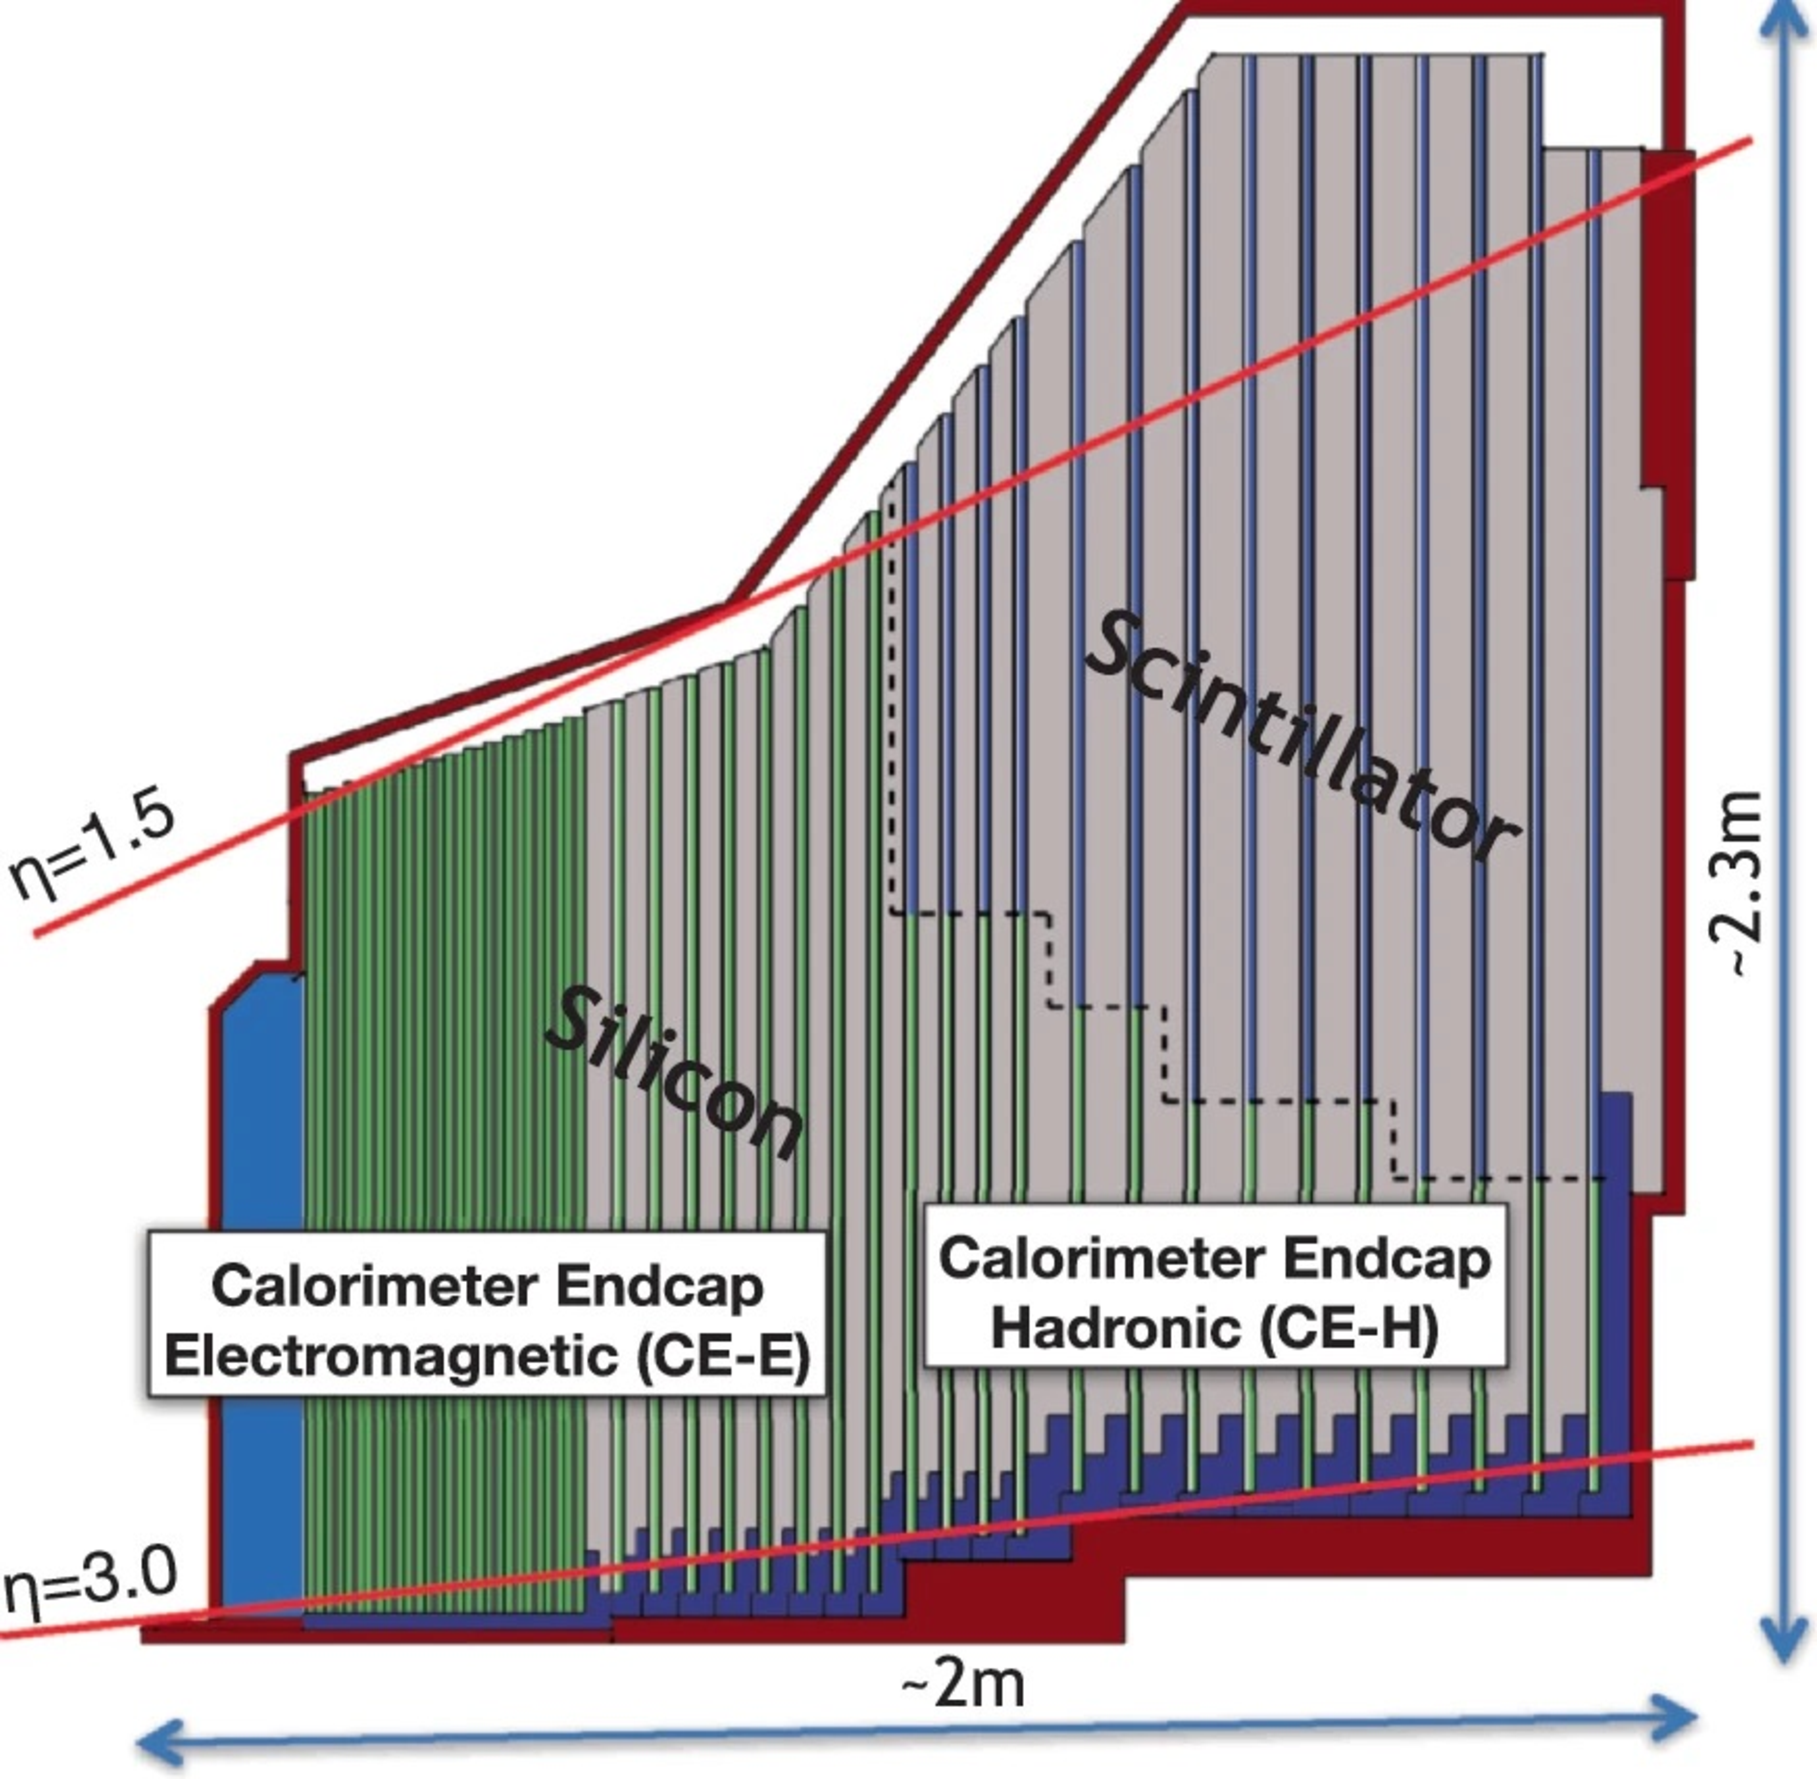
\includegraphics[width=\textwidth]{figures/02-CMS/cms/phase2/hgcal_layout}
    \caption{Layout of the CMS HGCAL, reproduced from Ref.~\cite{Quast2021}.}
    \label{fig:02_cms_hgcal}
\end{figure}

\begin{figure}[ht]
    \centering
    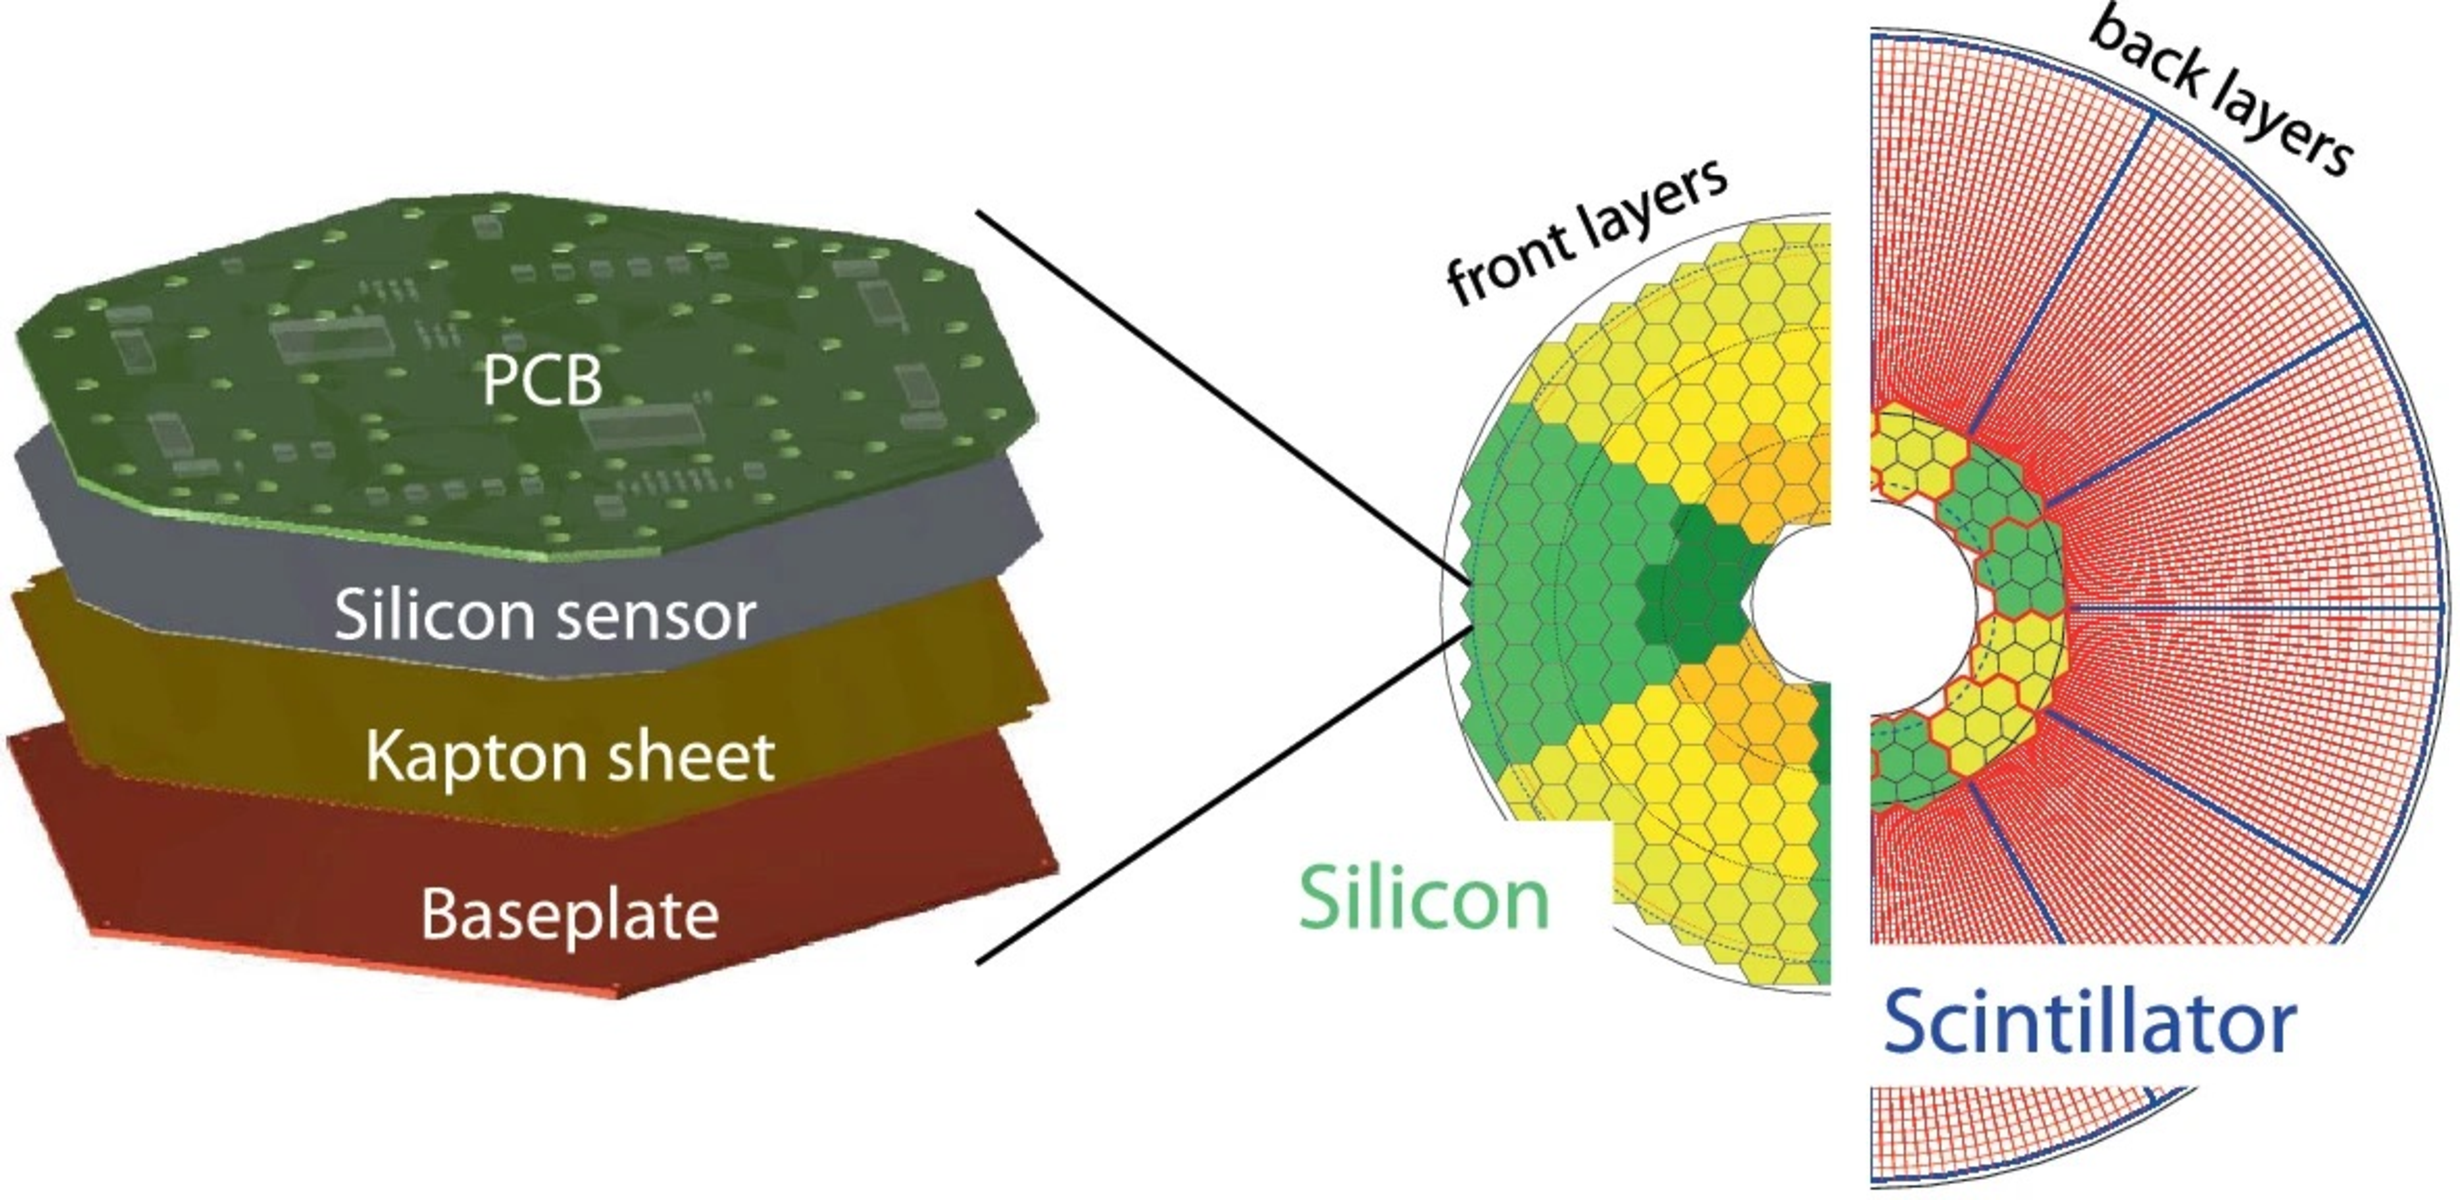
\includegraphics[width=\textwidth]{figures/02-CMS/cms/phase2/hgcal_sensors}
    \caption{(Left) layers of the individual HGCAL modules and (right) their layout in the all-silicon and mixed layers, reproduced from Ref.~\cite{Quast2021}.}
    \label{fig:02_cms_hgcal_sensors}
\end{figure}

Overall, the high-granularity, high-density, and fast timing calorimetry of the HGCAL is expected to significantly improve electron, photon, and jet efficiency and resolution, mitigate pileup, and allow more powerful trigger algorithms in HL-LHC~\cite{CMS:2017jpq}.
However, the increased complexity and occupancy, and unorthodox geometry, will pose significant challenges not only in its design and construction, but also computationally with respect to its simulation and reconstruction.
This is a strong motivation for the exploration of new computing techniques for fast and efficient CMS simulations, as we will discuss in Part~\ref{part:ml4sim}.

\subsection{Muon system}

As with the barrel calorimeters, the gas detectors themselves in the muon system are expected to continue performing well at the HL-LHC with no significant degradation in the overall muon reconstruction performance~\cite{CMS:2018rym}.
The electronics, however, will be upgraded to be more radiation hard and sustain the higher trigger rate.

The higher radiation and pileup does pose considerable challenges to reliable muon triggering in the very forward regions, however.
In fact, trigger inefficiencies were already anticipated in Run 3 of the LHC, which led to the installation of a new gas electron multiplier (GEM) station in the endcap regions of the muon system in the 2019--2022 long shutdown before Run 3, and recently another GEM station at the beginning of 2024~\cite{Calzaferri:2912038}.
GEMs are popular gas detectors with high rate capability and radiation tolerance, and provide crucial additional hit information to improve the trigger efficiency and muon reconstruction in the forward $1.5 < \abs{\eta} < 2.4$ regions.

During LS3, two more RPC stations for $1.8 < \abs{\eta} < 2.4$ and one final GEM will be added in the endcap regions for HL-LHC.
The RPCs will provide further forward timing information as well to complement the CSCs and recover single-muon trigger efficiencies~\cite{Pellecchia:2023aev}.
